% Created 2023-12-07 Πεμ 14:47
% Intended LaTeX compiler: pdflatex
\documentclass[11pt]{article}
\usepackage[utf8]{inputenc}
\usepackage[T1]{fontenc}
\usepackage{graphicx}
\usepackage{longtable}
\usepackage{wrapfig}
\usepackage{rotating}
\usepackage[normalem]{ulem}
\usepackage{amsmath}
\usepackage{amssymb}
\usepackage{capt-of}
\usepackage{hyperref}
\usepackage{booktabs}
\usepackage{import}
\usepackage[LGR, T1]{fontenc}
\usepackage[greek, english, american]{babel}
\usepackage{alphabeta}
\usepackage{esint}
\usepackage{mathtools}
\usepackage{esdiff}
\usepackage{makeidx}
\usepackage{glossaries}
\usepackage{newfloat}
\usepackage{minted}
\usepackage[a4paper, margin=3cm]{geometry}
\usepackage{chemfig}
\usepackage{svg}
\author{Βιδιάνος Γιαννίτσης}
\date{\today}
\title{Επεξεργασία δεδομένων της HPLC}
\hypersetup{
 pdfauthor={Βιδιάνος Γιαννίτσης},
 pdftitle={Επεξεργασία δεδομένων της HPLC},
 pdfkeywords={},
 pdfsubject={},
 pdfcreator={Emacs 29.1 (Org mode 9.6.6)}, 
 pdflang={English}}
\makeatletter
\newcommand{\citeprocitem}[2]{\hyper@linkstart{cite}{citeproc_bib_item_#1}#2\hyper@linkend}
\makeatother

\usepackage[notquote]{hanging}
\begin{document}

\maketitle
\tableofcontents

\begin{abstract}
Καθώς η διεργασία που μελετάμε είναι μία διεργασία ταυτόχρονης υδρόλυσης και ζύμωσης, είναι πολύ σημαντικό να κάνουμε monitor την ποσότητα σακχάρων αλλά και μεταβολικών προιόντων (πχ αιθανόλη και οργανικά οξέα). Η υγρή χρωματογραφία υψηλής απόδοσης (HPLC) είναι μία τέτοια τεχνική. Βέβαια, τα ακατέργαστα δεδομένα της είναι πίνακες με επιφάνειες στο χρωματογράφημα και θέλει μία επεξεργασία για να γίνει χρήσιμη. Σκοπός του αρχείου αυτού είναι να είναι ένα ολοκληρωμένο literate document το οποίο επεξηγεί την διαδικασία επεξεργασίας δεδομένων η οποία χρειάζεται. Κατά την λογική του literate programming, αυτό το αρχείο κάνει tangle τα σωστά scripts στον κατάλληλο φάκελο για να μπορούν να χρησιμοποιηθούν, αλλά μπορεί να τα κάνει και weave μέσα στο text σε ένα pdf format για καλύτερη επεξήγηση. Αξίζει να αναφερθεί πως γίνεται έντονη named code blocks τα οποία βοηθάνε στο να τρέξουμε πολλές φορές το ίδιο code block με βάση του noweb syntax που προσφέρει το org-mode. Καθώς το όνομα του code block δεν γίνεται weaved, θα υπάρχει με bold το όνομα πριν ακριβώς από κάθε code block, ώστε να μπορεί να κατανοηθεί και πότε κάποιο γίνεται inserted σε άλλα. Το αρχείο αυτό μπορεί να διαβαστεί στην μορφή ενός org document, το οποίο είναι το αρχικό document από τα οποία παράγονται και τα υπόλοιπα και διαβάζεται καλύτερα μέσω του Emacs, ως pdf το οποίο γίνεται weaved από το original και περιέχει όλη την πληροφορία του αρχικού χωρίς μόνο το interactivity και τέλος στην μορφή του κώδικα χωρίς τον σχολιασμό μέσω του tangled source code στο scripts directory.
\end{abstract}

\section{Dependencies}
\label{sec:orgea66a44}
Καθώς το project αυτό είναι δομημένο με το πακέτο DrWatson της Julia για να κάνει facilitate reproducibility, πρέπει σε όλα τα αρχεία να υπάρχουν τα lines που ενεργοποιούν το DrWatson και πηγαίνουν στο κατάλληλο project. Έπειτα, είναι επίσης απαραίτητο να κάνουμε include κάποια functions για την ανάλυση των δεδομένων το οποίο υπάρχει στο src directory και είναι amply documented εκεί.

\textbf{dependencies}
\begin{minted}[breaklines=true,breakanywhere=true]{julia}
using DrWatson
@quickactivate "Masters_Thesis"
include(srcdir("hplc_analysis.jl"))
\end{minted}

\section{Δημιουργία των πινάκων συγκεντρώσεων}
\label{sec:orgc329587}
Όπως αναφέρθηκε, τα ακατέργαστα δεδομένα της HPLC είναι πίνακες με επιφάνειες. Στο αρχείο \texttt{hplc\_analysis.jl} υπάρχουν τα helper functions που μετατρέπουν την επιφάνεια σε συγκέντρωση, ένα function (\texttt{process\_area\_data}) που κάνει bundle όλα αυτά μαζί και ένα ακόμη που διαβάζει το area, τρέχει το function της επεξεργασίας, αποθηκεύει την συγκέντρωση και την διαβάζει. Έτσι, μπορούμε σχετικά εύκολα με μία γραμμή κώδικα να κάνουμε την μετατροπή. Για να είναι πιο εύκολα reproducible το code block αυτό, υπάρχουν και τα functions \texttt{get\_area\_csv} και \texttt{get\_conc\_csv} τα οποία αν τους δωθεί ένα date και ποσότητα ενζύμου, βρίσκουν το κατάλληλο csv που πρέπει να διαβαστεί/αποθηκευτεί. Έτσι, αλλάζοντας την ημερομηνία, μπορούμε να διαβάσουμε διαφορετικά δεδομένα και να κάνουμε build τον κώδικα accordingly. Παρακάτω φαίνεται αυτή η διαδικασία για τα βασικά μας πειράματα.

\subsection{Πείραμα 10-11}
\label{sec:org6605812}
Το πείραμα κωδικοποιημένο ως πείραμα 10-11 (που στην πραγματικότητα έτρεξε όλη την εβδομάδα που ξεκίνησε από τις 6-11 και τελείωσε στις 10) είναι το πρώτο πείραμα δοκιμής διαφορετικών ποσοτήτων mix. Χρησιμοποιήθηκαν τα ένζυμα PROGEN σε ποσότητες 0, 1, 2, 4 και 8 ml για την επεξεργασία δειγμάτων με 200 g FW και 600 g νερό. Η θερμοκρασία ρυθμίστηκε με θερμοστάτη στους 35 \(^oC\).

Στο πείραμα αυτό έγιναν δειγματοληψίες στις 0, 24, 48 και 72 ώρες για να δούμε την πρόοδο της αντίδρασης με βασικό εργαλείο την μέτρηση της HPLC αλλά και μετρήσεις pH και αγωγιμότητας. Στο παρακάτω code block διαβάζονται τα αντίστοιχα δεδομένα.

\textbf{area\textsubscript{to}\textsubscript{conc}\textsubscript{10}\textsubscript{11}}
\begin{minted}[breaklines=true,breakanywhere=true]{julia}
date = "10_11"
mix_amount = ["0", "1", "2", "4", "8"]
t = [0, 24, 48, 72]

df0_conc = process_area_data(get_area_csv(date, mix_amount[1]), get_conc_csv(date, mix_amount[1]))
df1_conc = process_area_data(get_area_csv(date, mix_amount[2]), get_conc_csv(date, mix_amount[2]))
df2_conc = process_area_data(get_area_csv(date, mix_amount[3]), get_conc_csv(date, mix_amount[3]))
df4_conc = process_area_data(get_area_csv(date, mix_amount[4]), get_conc_csv(date, mix_amount[4]))
df8_conc = process_area_data(get_area_csv(date, mix_amount[5]), get_conc_csv(date, mix_amount[5]))

\end{minted}

\subsection{Πείραμα 28-11}
\label{sec:orgf733b91}
Το πείραμα κωδικοποιημένο ως πείραμα 28-11 έτρεξε στην πραγματικότητα 21-24/11 όμως τα αποτελέσματα της HPLC τα πήραμε στις 28 και για αυτό τα αντίστοιχα files έχουν αυτήν την ημερομηνία η οποία χρησιμοποιείται στην κωδικοποίηση. Το πείραμα αυτό ήταν ακριβώς αντίστοιχο με το παραπάνω με μόνη διαφορά ότι εξετάστηκε άλλη θερμοκρασία, η οποία ήταν στους 40 \(^oC\). Το code block παρακάτω είναι μία αντιγραφή του προηγούμενου με μόνη διαφορά ότι έχει αλλάξει η τιμή του variable date το οποίο ελέγχει από που θα διαβαστούν τα δεδομένα.

\textbf{area\textsubscript{to}\textsubscript{conc}\textsubscript{28}\textsubscript{11}}
\begin{minted}[breaklines=true,breakanywhere=true]{julia}
date = "28_11"
mix_amount = ["0", "1", "2", "4", "8"]
t = [0, 24, 48, 72]

df0_conc = process_area_data(get_area_csv(date, mix_amount[1]), get_conc_csv(date, mix_amount[1]))
df1_conc = process_area_data(get_area_csv(date, mix_amount[2]), get_conc_csv(date, mix_amount[2]))
df2_conc = process_area_data(get_area_csv(date, mix_amount[3]), get_conc_csv(date, mix_amount[3]))
df4_conc = process_area_data(get_area_csv(date, mix_amount[4]), get_conc_csv(date, mix_amount[4]))
df8_conc = process_area_data(get_area_csv(date, mix_amount[5]), get_conc_csv(date, mix_amount[5]))

\end{minted}

\subsection{Πείραμα 23-10}
\label{sec:orgbba45ae}
Το πείραμα 23-10 ήταν το αρχικό πείραμα που εξετάστηκε κάνοντας μία κινητική ανάλυση του πειράματος για να καταλάβουμε πως λειτουργεί και πως θα σχεδιάσουμε τα επόμενα πειράματα. Για το πείραμα αυτό επιλέχθηκε η θερμοκρασία 45 \(^oC\) και η ποσότητα 2 ml από το mix. Έγιναν 2 επαναλήψεις του πειράματος οι οποίες διέφεραν κυρίως στην πρώτη μέρα. Στο ένα πάρθηκε δείγμα κάθε ώρα για τις πρώτες 6 ώρες ενώ στο 2ο στις 0, 1 και 5 ώρες. Για την υπόλοιπη εβδομάδα εκείνη παίρναμε 3 δείγματα την μέρα με 2 ώρες απόσταση μεταξύ τους και έπειτα το δείγμα αφέθηκε όλο το σαββατοκύριακο και πάρθηκαν 2 τελικά δείγματα την επόμενη δευτέρα με 4 ώρες απόσταση μεταξύ τους. Έτσι, είχαμε μία αρκετά πιο ολοκληρωμένη εικόνα η οποία βοήθησε στον σχεδιασμό των άλλων πειραμάτων. Βέβαια, για την επεξεργασία των δεδομένων αυτών χρειάζεται ένα διαφορετικό approach που φαίνεται εδώ.

\textbf{area\textsubscript{to}\textsubscript{conc}\textsubscript{23}\textsubscript{10}}
\begin{minted}[breaklines=true,breakanywhere=true]{julia}
date = "23_10"
df2310_1_conc = process_area_data2(get_area_csv(date, "1"), get_conc_csv(date, "1"))
t1 = df2310_1_conc.Time

df2310_2_conc = process_area_data2(get_area_csv(date, "2"), get_conc_csv(date, "2"))
t2 = df2310_2_conc.Time
\end{minted}

\section{Δημιουργία Scatter Plots}
\label{sec:org891e401}
Έχοντας διαβάσει τα παραπάνω δεδομένα, μπορούμε να αρχίσουμε να κάνουμε διαγράμματα. Ένα πρώτο παράδειγμα είναι scatter plots. Τα παρακάτω code blocks είναι φτιαγμένα ώστε να βασίζονται στα data frames και το variable date που διαβάστηκαν παραπάνω έτσι ώστε αν καλεστούν sequentially με κάποιο από τα παραπάνω να παραχθούν τα κατάλληλα διαγράμματα. Το helper function \texttt{get\_plot\_name} που υπάρχει στο src directory κάνει facilitate αυτή τη συμπεριφορά κάνοντας εύκολη την δημιουργία των file names από το variable date, το είδος της ένωσης και το plot type που κάνουμε. Αυτά τα blocks είναι για τα πειράματα 10 και 28 Νοεμβρίου τα οποία έχουν το ίδιο format και όποιο άλλο γίνει πιθανόν με την ίδια λογική.

\subsection{Scatters ανά ποσότητα mix}
\label{sec:orgeaf4790}
Αρχικά, δοκιμάστηκε να φτιαχτούν κάποια scatter plots όπου το κάθε χρώμα αντιστοιχεί σε μία ποσότητα mix και στο κάθε διάγραμμα υπάρχει μία ένωση

\textbf{scatter\textsubscript{plots}}
\begin{minted}[breaklines=true,breakanywhere=true]{julia}
plot_type = "scatter"
plot_label = ["0 ml" "1 ml" "2 ml" "4 ml" "8 ml"]

suc_scatter = scatter(t, [df0_conc.Sucrose df1_conc.Sucrose df2_conc.Sucrose df4_conc.Sucrose df8_conc.Sucrose], label = plot_label,
                    xticks = t, title = "Sucrose Concentration",
                    xlabel = "Time (h)", ylabel = "Sucrose (g/l)", markersize = 6)
savefig(suc_scatter, get_plot_name("sucrose", date, plot_type))

gluc_scatter = scatter(t, [df0_conc.Glucose df1_conc.Glucose df2_conc.Glucose df4_conc.Glucose df8_conc.Glucose], label = plot_label,
                       xticks = t, title = "Glucose Concentration",
                       xlabel = "Time (h)", ylabel = "Glucose (g/l)", markersize = 6)
savefig(gluc_scatter, get_plot_name("glucose", date, plot_type))

fruc_scatter = scatter(t, [df0_conc.Fructose df1_conc.Fructose df2_conc.Fructose df4_conc.Fructose df8_conc.Fructose], label = plot_label,
                       xticks = t, title = "Fructose Concentration",
                       xlabel = "Time (h)", ylabel = "Fructose (g/l)", markersize = 6)
savefig(fruc_scatter, get_plot_name("fructose", date, plot_type))

lact_scatter = scatter(t, [df0_conc.Lactate df1_conc.Lactate df2_conc.Lactate df4_conc.Lactate df8_conc.Lactate], label = plot_label,
                       xticks = t, title = "Lactate Concentration",
                       xlabel = "Time (h)", ylabel = "Lactate (g/l)", markersize = 6)
savefig(lact_scatter, get_plot_name("lactate", date, plot_type))

ac_scatter = scatter(t, [df0_conc.Acetate df1_conc.Acetate df2_conc.Acetate df4_conc.Acetate df8_conc.Acetate], label = plot_label,
                     xticks = t, title = "Acetate Concentration",
                     xlabel = "Time (h)", ylabel = "Acetate (g/l)", markersize = 6)
savefig(ac_scatter, get_plot_name("acetate", date, plot_type))

prop_scatter = scatter(t, [df0_conc.Propionate df1_conc.Propionate df2_conc.Propionate df4_conc.Propionate df8_conc.Propionate], label = plot_label,
                       xticks = t, title = "Propionate Concentration",
                       xlabel = "Time (h)", ylabel = "Propionate (g/l)", markersize = 6)
savefig(prop_scatter, get_plot_name("propionate", date, plot_type))

eth_scatter = scatter(t, [df0_conc.Ethanol df1_conc.Ethanol df2_conc.Ethanol df4_conc.Ethanol df8_conc.Ethanol], label = plot_label,
                      xticks = t, title = "Ethanol Concentration",
                      xlabel = "Time (h)", ylabel = "Ethanol (g/l)", markersize = 6)
savefig(eth_scatter, get_plot_name("ethanol", date, plot_type))

pH_scatter = scatter(t, [df0_conc.pH df1_conc.pH df2_conc.pH df4_conc.pH df8_conc.pH], label = plot_label,
                     xticks = t, title = "pH-t",
                     xlabel = "Time (h)", ylabel = "pH", markersize = 6)
savefig(pH_scatter, get_plot_name("pH", date, plot_type))

scatter_final = plot(suc_scatter, gluc_scatter, fruc_scatter,
                         lact_scatter, ac_scatter, prop_scatter,
                         eth_scatter, pH_scatter,
                         layout = 9, size = (1350, 900))
savefig(scatter_final, get_plot_name("final", date, plot_type))

\end{minted}

\subsection{Scatter ανά δείγμα}
\label{sec:org83abc51}
Ένας εναλλακτικός τρόπος να δείξουμε τα δεδομένα όμως είναι όλες οι ενώσεις κάθε δείγματος μαζί αντί για όλα τα δείγματα μαζί για κάθε ένωση, έχοντας δηλαδή ένα διάγραμμα ανά ποσότητα mix και όλες τις ενώσεις ως διαφορετικά χρώματα σε αυτό.

\textbf{conc\textsubscript{scatter}\textsubscript{plots}}
\begin{minted}[breaklines=true,breakanywhere=true]{julia}
plot_type = "scatter"

conc_scatter_0 = scatter(t, [df0_conc.Sucrose df0_conc.Glucose df0_conc.Fructose df0_conc.Lactate df0_conc.Acetate df0_conc.Propionate df0_conc.Ethanol],
                         label = ["Sucrose" "Glucose" "Fructose" "Lactate" "Acetate" "Propionate" "Ethanol"], xticks = t, title = "Concentrations for sample with 0 mL mix", xlabel = "Time (h)", ylabel = "Concentration (g/l)",
                         markersize = 6)
savefig(conc_scatter_0, get_plot_name("conc_0", date, plot_type))

conc_scatter_1 = scatter(t, [df1_conc.Sucrose df1_conc.Glucose df1_conc.Fructose df1_conc.Lactate df1_conc.Acetate df1_conc.Propionate df1_conc.Ethanol],
                         label = ["Sucrose" "Glucose" "Fructose" "Lactate" "Acetate" "Propionate" "Ethanol"], xticks = t, title = "Concentrations for sample with 1 mL mix", xlabel = "Time (h)", ylabel = "Concentration (g/l)",
                         markersize = 6)
savefig(conc_scatter_1, get_plot_name("conc_1", date, plot_type))

conc_scatter_2 = scatter(t, [df2_conc.Sucrose df2_conc.Glucose df2_conc.Fructose df2_conc.Lactate df2_conc.Acetate df2_conc.Propionate df2_conc.Ethanol],
                         label = ["Sucrose" "Glucose" "Fructose" "Lactate" "Acetate" "Propionate" "Ethanol"], xticks = t, title = "Concentrations for sample with 2 mL mix", xlabel = "Time (h)", ylabel = "Concentration (g/l)",
                         markersize = 6)
savefig(conc_scatter_2, get_plot_name("conc_2", date, plot_type))

conc_scatter_4 = scatter(t, [df4_conc.Sucrose df4_conc.Glucose df4_conc.Fructose df4_conc.Lactate df4_conc.Acetate df4_conc.Propionate df4_conc.Ethanol],
                         label = ["Sucrose" "Glucose" "Fructose" "Lactate" "Acetate" "Propionate" "Ethanol"], xticks = t, title = "Concentrations for sample with 4 mL mix", xlabel = "Time (h)", ylabel = "Concentration (g/l)",
                         markersize = 6)
savefig(conc_scatter_4, get_plot_name("conc_4", date, plot_type))

conc_scatter_8 = scatter(t, [df8_conc.Sucrose df8_conc.Glucose df8_conc.Fructose df8_conc.Lactate df8_conc.Acetate df8_conc.Propionate df8_conc.Ethanol],
                         label = ["Sucrose" "Glucose" "Fructose" "Lactate" "Acetate" "Propionate" "Ethanol"], xticks = t, title = "Concentrations for sample with 8 mL mix", xlabel = "Time (h)", ylabel = "Concentration (g/l)",
                         markersize = 6)
savefig(conc_scatter_8, get_plot_name("conc_8", date, plot_type))

conc_scatter = scatter(conc_scatter_0, conc_scatter_1, conc_scatter_2, conc_scatter_4, conc_scatter_8, layout = 5, size = (1500, 900))
savefig(conc_scatter, get_plot_name("conc", date, plot_type))

\end{minted}

\subsection{Scatter Plots για κινητική}
\label{sec:org657d4c2}
Όπως αναφέρθηκε και προηγουμένως, το κινητικό πείραμα στις 23/10 είχε διαφορετικό formatting, οπότε χρειάζεται ελαφρώς διαφορετικό κώδικα. Καθώς αυτό το πείραμα έγινε μόνο μία φορά βάζουμε και το code block που διαβάζει τα δεδομένα μέσα σε αυτό με το noweb syntax.

\textbf{scatter\textsubscript{23}\textsubscript{10}}
\begin{minted}[breaklines=true,breakanywhere=true]{julia}
<<area_to_conc_23_10>>

plot_type = "scatter"

suc_scatter = scatter(t1, [df2310_1_conc.Sucrose], label = "1", title = "Sucrose Concentration",
                      xlabel = "Time (h)", ylabel = "Sucrose (g/l)", markersize = 6)
scatter!(t2, df2310_2_conc.Sucrose, label = "2", markersize = 6)
savefig(suc_scatter, get_plot_name("sucrose", date, plot_type))

gluc_scatter = scatter(t1, [df2310_1_conc.Glucose], label = "1", title = "Glucose Concentration",
                      xlabel = "Time (h)", ylabel = "Glucose (g/l)", markersize = 6)
scatter!(t2, df2310_2_conc.Glucose, label = "2", markersize = 6)
savefig(gluc_scatter, get_plot_name("glucose", date, plot_type))

fruc_scatter = scatter(t1, [df2310_1_conc.Fructose], label = "1", title = "Fructose Concentration",
                      xlabel = "Time (h)", ylabel = "Fructose (g/l)", markersize = 6)
scatter!(t2, df2310_2_conc.Fructose, label = "2", markersize = 6)
savefig(fruc_scatter, get_plot_name("fructose", date, plot_type))

lact_scatter = scatter(t1, [df2310_1_conc.Lactate], label = "1", title = "Lactate Concentration",
                      xlabel = "Time (h)", ylabel = "Lactate (g/l)", markersize = 6)
scatter!(t2, df2310_2_conc.Lactate, label = "2", markersize = 6)
savefig(lact_scatter, get_plot_name("lactate", date, plot_type))

ac_scatter = scatter(t1, [df2310_1_conc.Acetate], label = "1", title = "Acetate Concentration",
                      xlabel = "Time (h)", ylabel = "Acetate (g/l)", markersize = 6)
scatter!(t2, df2310_2_conc.Acetate, label = "2", markersize = 6)
savefig(ac_scatter, get_plot_name("acetate", date, plot_type))

prop_scatter = scatter(t1, [df2310_1_conc.Propionate], label = "1", title = "Propionate Concentration",
                      xlabel = "Time (h)", ylabel = "Propionate (g/l)", markersize = 6)
scatter!(t2, df2310_2_conc.Propionate, label = "2", markersize = 6)
savefig(prop_scatter, get_plot_name("propionate", date, plot_type))

eth_scatter = scatter(t1, [df2310_1_conc.Ethanol], label = "1", title = "Ethanol Concentration",
                      xlabel = "Time (h)", ylabel = "Ethanol (g/l)", markersize = 6)
scatter!(t2, df2310_2_conc.Ethanol, label = "2", markersize = 6)
savefig(eth_scatter, get_plot_name("ethanol", date, plot_type))

scatter_final = plot(suc_scatter, gluc_scatter, fruc_scatter,
                         lact_scatter, ac_scatter, prop_scatter,
                         eth_scatter, layout = 9, size = (1350, 900))
savefig(scatter_final, get_plot_name("final", date, plot_type))

\end{minted}

\section{Δημιουργία bar plots}
\label{sec:org38b8140}
Βέβαια, ένας εναλλακτικός τρόπος να δείξουμε τα ίδια δεδομένα είναι και μέσω μπαρών, οι οποίες είναι ίσως πιο ωραίες σε κάποιες περιπτώσεις. Ο κώδικας είναι σχεδόν ίδιος, με την βασική διαφορά πως γίνεται χρήση του \texttt{groupedbar} από το \texttt{StatsPlots.jl} αντί για το \texttt{scatter} του βασικού \texttt{Plots.jl}. 

\subsection{Bar plots άνα δείγμα}
\label{sec:orge729fb4}

\textbf{bar\textsubscript{plots}}
\begin{minted}[breaklines=true,breakanywhere=true]{julia}
plot_type = "bar"
plot_label = ["0 ml" "1 ml" "2 ml" "4 ml" "8 ml"]

suc_groupedbar = groupedbar(t, [df0_conc.Sucrose df1_conc.Sucrose df2_conc.Sucrose df4_conc.Sucrose df8_conc.Sucrose], label = plot_label,
                    xticks = t, title = "Sucrose Concentration",
                    xlabel = "Time (h)", ylabel = "Sucrose (g/l)", markersize = 6)
savefig(suc_groupedbar, get_plot_name("sucrose", date, plot_type))

gluc_groupedbar = groupedbar(t, [df0_conc.Glucose df1_conc.Glucose df2_conc.Glucose df4_conc.Glucose df8_conc.Glucose], label = plot_label,
                       xticks = t, title = "Glucose Concentration",
                       xlabel = "Time (h)", ylabel = "Glucose (g/l)", markersize = 6)
savefig(gluc_groupedbar, get_plot_name("glucose", date, plot_type))

fruc_groupedbar = groupedbar(t, [df0_conc.Fructose df1_conc.Fructose df2_conc.Fructose df4_conc.Fructose df8_conc.Fructose], label = plot_label,
                       xticks = t, title = "Fructose Concentration",
                       xlabel = "Time (h)", ylabel = "Fructose (g/l)", markersize = 6)
savefig(fruc_groupedbar, get_plot_name("fructose", date, plot_type))

lact_groupedbar = groupedbar(t, [df0_conc.Lactate df1_conc.Lactate df2_conc.Lactate df4_conc.Lactate df8_conc.Lactate], label = plot_label,
                       xticks = t, title = "Lactate Concentration",
                       xlabel = "Time (h)", ylabel = "Lactate (g/l)", markersize = 6)
savefig(lact_groupedbar, get_plot_name("lactate", date, plot_type))

ac_groupedbar = groupedbar(t, [df0_conc.Acetate df1_conc.Acetate df2_conc.Acetate df4_conc.Acetate df8_conc.Acetate], label = plot_label,
                     xticks = t, title = "Acetate Concentration",
                     xlabel = "Time (h)", ylabel = "Acetate (g/l)", markersize = 6)
savefig(ac_groupedbar, get_plot_name("acetate", date, plot_type))

prop_groupedbar = groupedbar(t, [df0_conc.Propionate df1_conc.Propionate df2_conc.Propionate df4_conc.Propionate df8_conc.Propionate], label = plot_label,
                       xticks = t, title = "Propionate Concentration",
                       xlabel = "Time (h)", ylabel = "Propionate (g/l)", markersize = 6)
savefig(prop_groupedbar, get_plot_name("propionate", date, plot_type))

eth_groupedbar = groupedbar(t, [df0_conc.Ethanol df1_conc.Ethanol df2_conc.Ethanol df4_conc.Ethanol df8_conc.Ethanol], label = plot_label,
                      xticks = t, title = "Ethanol Concentration",
                      xlabel = "Time (h)", ylabel = "Ethanol (g/l)", markersize = 6)
savefig(eth_groupedbar, get_plot_name("ethanol", date, plot_type))

pH_groupedbar = groupedbar(t, [df0_conc.pH df1_conc.pH df2_conc.pH df4_conc.pH df8_conc.pH], label = plot_label,
                     xticks = t, title = "pH-t",
                     xlabel = "Time (h)", ylabel = "pH", markersize = 6)
savefig(pH_groupedbar, get_plot_name("pH", date, plot_type))

groupedbar_final = plot(suc_groupedbar, gluc_groupedbar, fruc_groupedbar,
                         lact_groupedbar, ac_groupedbar, prop_groupedbar,
                         eth_groupedbar, pH_groupedbar,
                         layout = 9, size = (1350, 900))
savefig(groupedbar_final, get_plot_name("final", date, plot_type))

\end{minted}

\subsection{Bar plots άνα δείγμα}
\label{sec:orga851530}

\textbf{conc\textsubscript{bar}\textsubscript{plots}}
\begin{minted}[breaklines=true,breakanywhere=true]{julia}
plot_type = "bar"

conc_groupedbar_0 = groupedbar(t, [df0_conc.Sucrose df0_conc.Glucose df0_conc.Fructose df0_conc.Lactate df0_conc.Acetate df0_conc.Propionate df0_conc.Ethanol],
                               label = ["Sucrose" "Glucose" "Fructose" "Lactate" "Acetate" "Propionate" "Ethanol"], xticks = t, title = "Concentrations for sample with 0 mL mix", xlabel = "Time (h)", ylabel = "Concentration (g/l)",
                         markersize = 6)
savefig(conc_groupedbar_0, get_plot_name("conc_0", date, plot_type))

conc_groupedbar_1 = groupedbar(t, [df1_conc.Sucrose df1_conc.Glucose df1_conc.Fructose df1_conc.Lactate df1_conc.Acetate df1_conc.Propionate df1_conc.Ethanol],
                               label = ["Sucrose" "Glucose" "Fructose" "Lactate" "Acetate" "Propionate" "Ethanol"], xticks = t, title = "Concentrations for sample with 1 mL mix", xlabel = "Time (h)", ylabel = "Concentration (g/l)",
                               markersize = 6)
savefig(conc_groupedbar_1, get_plot_name("conc_1", date, plot_type))

conc_groupedbar_2 = groupedbar(t, [df2_conc.Sucrose df2_conc.Glucose df2_conc.Fructose df2_conc.Lactate df2_conc.Acetate df2_conc.Propionate df2_conc.Ethanol],
                               label = ["Sucrose" "Glucose" "Fructose" "Lactate" "Acetate" "Propionate" "Ethanol"], xticks = t, title = "Concentrations for sample with 2 mL mix", xlabel = "Time (h)", ylabel = "Concentration (g/l)",
                               markersize = 6)
savefig(conc_groupedbar_2, get_plot_name("conc_2", date, plot_type))

conc_groupedbar_4 = groupedbar(t, [df4_conc.Sucrose df4_conc.Glucose df4_conc.Fructose df4_conc.Lactate df4_conc.Acetate df4_conc.Propionate df4_conc.Ethanol],
                               label = ["Sucrose" "Glucose" "Fructose" "Lactate" "Acetate" "Propionate" "Ethanol"], xticks = t, title = "Concentrations for sample with 4 mL mix", xlabel = "Time (h)", ylabel = "Concentration (g/l)",
                               markersize = 6)
savefig(conc_groupedbar_4, get_plot_name("conc_4", date, plot_type))

conc_groupedbar_8 = groupedbar(t, [df8_conc.Sucrose df8_conc.Glucose df8_conc.Fructose df8_conc.Lactate df8_conc.Acetate df8_conc.Propionate df8_conc.Ethanol],
                               label = ["Sucrose" "Glucose" "Fructose" "Lactate" "Acetate" "Propionate" "Ethanol"], xticks = t, title = "Concentrations for sample with 8 mL mix", xlabel = "Time (h)", ylabel = "Concentration (g/l)",
                               markersize = 6)
savefig(conc_groupedbar_8, get_plot_name("conc_8", date, plot_type))

conc_groupedbar = plot(conc_groupedbar_0, conc_groupedbar_1, conc_groupedbar_2, conc_groupedbar_4, conc_groupedbar_8, layout = 5, size = (1500, 900))
savefig(conc_groupedbar, get_plot_name("conc", date, plot_type))

\end{minted}

\section{Συγκριτικά bar plots μεταξύ των πειραμάτων}
\label{sec:org30e258b}
Μία άλλη ιδέα είναι αντί για να συγκρίνουμε τις ποσότητες, να συγκρίνουμε θερμοκρασίες για ίδια ποσότητα. Στα παρακάτω code blocks γίνεται αυτό ακριβώς, σε bar plot representation το οποίο θεωρήθηκε πιο ευανάγνωστο. 
\subsection{Συλλογή δεδομένων}
\label{sec:org81e70ad}
Καθώς αυτή η σύγκιση χρειάζεται να γίνει μόνο μία φορά για τα συγκεκριμένα πειράματα, ορίζονται explicitly και τα 3 data sets για να γίνει το plotting.

\textbf{comp\textsubscript{data}\textsubscript{collection}}
\begin{minted}[breaklines=true,breakanywhere=true]{julia}

<<area_to_conc_28_11>>
df2310_1_conc = CSV.read(datadir("exp_pro/hplc_conc_23_10_1_comp.csv"), DataFrame)
df2310_2_conc = CSV.read(datadir("exp_pro/hplc_conc_23_10_2_comp.csv"), DataFrame)

df1011_0_conc = CSV.read(datadir("exp_pro/hplc_conc_10_11_0.csv"), DataFrame)
df1011_1_conc = CSV.read(datadir("exp_pro/hplc_conc_10_11_1.csv"), DataFrame)
df1011_2_conc = CSV.read(datadir("exp_pro/hplc_conc_10_11_2.csv"), DataFrame)
df1011_4_conc = CSV.read(datadir("exp_pro/hplc_conc_10_11_4.csv"), DataFrame)
df1011_8_conc = CSV.read(datadir("exp_pro/hplc_conc_10_11_8.csv"), DataFrame)

\end{minted}

\subsection{Συγκριτικά διαγράμματα των 3 πειραμάτων}
\label{sec:orgc8fc742}
Αρχικά γίνεται για τα 2 ml mix, όπου έχουμε 4 διαφορετικά πειράματα, ένα στους 35, ένα στους 40 και 2 στούς 45. Καθώς αυτό το block φτιάχνει ένα μόνο τελικό διάγραμμα, φαίνεται παρακάτω και το αποτέλεσμα του.

\textbf{comp\textsubscript{plots}\textsubscript{2}\textsubscript{ml}}
\begin{minted}[breaklines=true,breakanywhere=true]{julia}

suc_groupedbar = groupedbar(t, [df1011_2_conc.Sucrose df2_conc.Sucrose df2310_1_conc.Sucrose df2310_2_conc.Sucrose], label = ["35 C" "40 C" "45 C (1)" "45 C (2)"],
                            xticks = t, title = "Sucrose Concentration",
                            xlabel = "Time (h)", ylabel = "Sucrose (g/l)")
savefig(suc_groupedbar, plotsdir("35_40_45_comp/sucrose_bar_comp_2.png"))

gluc_groupedbar = groupedbar(t, [df1011_2_conc.Glucose df2_conc.Glucose df2310_1_conc.Glucose df2310_2_conc.Glucose], label = ["35 C" "40 C" "45 C (1)" "45 C (2)"],
                             xticks = t, title = "Glucose Concentration",
                             xlabel = "Time (h)", ylabel = "Glucose (g/l)")
savefig(gluc_groupedbar, plotsdir("35_40_45_comp/glucose_bar_comp_2.png"))

fruc_groupedbar = groupedbar(t, [df1011_2_conc.Fructose df2_conc.Fructose df2310_1_conc.Fructose df2310_2_conc.Fructose], label = ["35 C" "40 C" "45 C (1)" "45 C (2)"],
                             xticks = t, title = "Fructose Concentration",
                             xlabel = "Time (h)", ylabel = "Fructose (g/l)")
savefig(fruc_groupedbar, plotsdir("35_40_45_comp/fructose_bar_comp_2.png"))

lact_groupedbar = groupedbar(t, [df1011_2_conc.Lactate df2_conc.Lactate df2310_1_conc.Lactate df2310_2_conc.Lactate], label = ["35 C" "40 C" "45 C (1)" "45 C (2)"],
                             xticks = t, title = "Lactate Concentration",
                             xlabel = "Time (h)", ylabel = "Lactate (g/l)")
savefig(lact_groupedbar, plotsdir("35_40_45_comp/lactate_bar_comp_2.png"))

ac_groupedbar = groupedbar(t, [df1011_2_conc.Acetate df2_conc.Acetate df2310_1_conc.Acetate df2310_2_conc.Acetate], label = ["35 C" "40 C" "45 C (1)" "45 C (2)"],
                           xticks = t, title = "Acetate Concentration",
                           xlabel = "Time (h)", ylabel = "Acetate (g/l)")
savefig(ac_groupedbar, plotsdir("35_40_45_comp/acetate_bar_comp_2.png"))

prop_groupedbar = groupedbar(t, [df1011_2_conc.Propionate df2_conc.Propionate df2310_1_conc.Propionate df2310_2_conc.Propionate], label = ["35 C" "40 C" "45 C (1)" "45 C (2)"],
                             xticks = t, title = "Propionate Concentration",
                             xlabel = "Time (h)", ylabel = "Propionate (g/l)", legend = :bottomleft)
savefig(prop_groupedbar, plotsdir("35_40_45_comp/propionate_bar_comp_2.png"))

eth_groupedbar = groupedbar(t, [df1011_2_conc.Ethanol df2_conc.Ethanol df2310_1_conc.Ethanol df2310_2_conc.Ethanol], label = ["35 C" "40 C" "45 C (1)" "45 C (2)"],
                            xticks = t, title = "Ethanol Concentration",
                            xlabel = "Time (h)", ylabel = "Ethanol (g/l)")
savefig(eth_groupedbar, plotsdir("35_40_45_comp/ethanol_bar_comp_2.png"))

grouped_bar_comp = plot(suc_groupedbar, gluc_groupedbar, fruc_groupedbar,
                         lact_groupedbar, ac_groupedbar, prop_groupedbar,
                         eth_groupedbar, layout = 7, size = (1400, 900))
savefig(grouped_bar_comp, plotsdir("35_40_45_comp/grouped_bar_comp_2.png"))

\end{minted}

\begin{figure}[htbp]
\centering
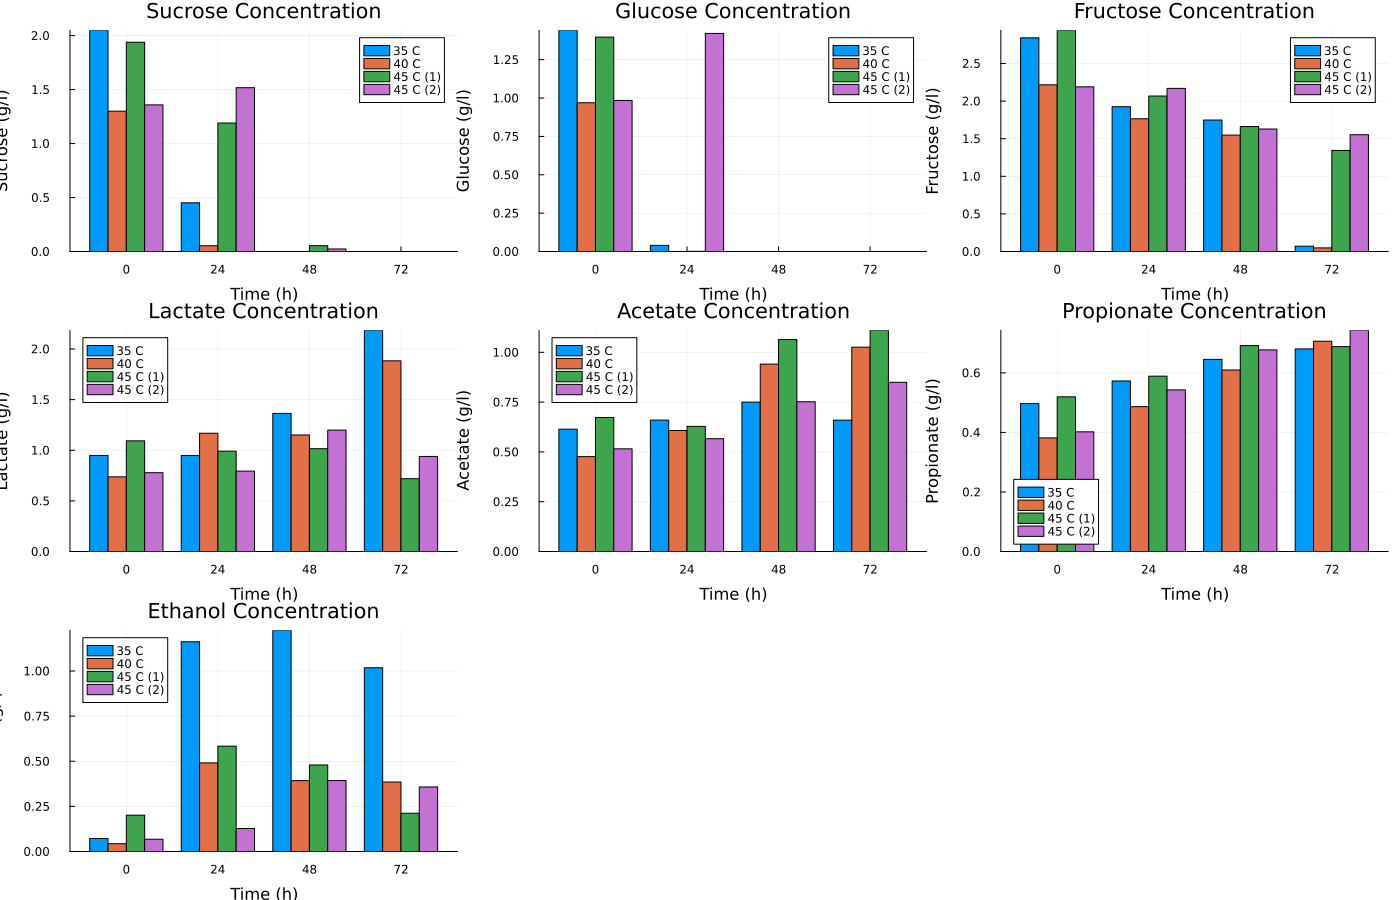
\includegraphics[width=.9\linewidth]{/home/vidianos/Documents/9o_εξάμηνο/Masters_Thesis/plots/35_40_45_comp/grouped_bar_comp_2.png}
\caption{Συγκριτικά διαγράμματα των 3 πειραμάτων στα 2 ml mix}
\end{figure}

\subsection{Συγκριτικά διαγράμματα των υπολοίπων ποσοτήτων}
\label{sec:orgb0797a7}
Και έπειτα γίνονται για τις υπόλοιπες ποσότητες συγκρίνοντας τους 35 με τους 40.

\textbf{comp\textsubscript{plots}\textsubscript{no}\textsubscript{kinetic}}
\begin{minted}[breaklines=true,breakanywhere=true]{julia}

suc_groupedbar_0 = groupedbar(t, [df0_conc.Sucrose df1011_0_conc.Sucrose], label = ["40 C" "35 C"],
                            xticks = t, title = "Sucrose Concentration",
                            xlabel = "Time (h)", ylabel = "Sucrose (g/l)")
savefig(suc_groupedbar_0, plotsdir("35_40_comp/sucrose_bar_comp_0.png"))

gluc_groupedbar_0 = groupedbar(t, [df0_conc.Glucose df1011_0_conc.Glucose], label = ["40 C" "35 C"],
                            xticks = t, title = "Glucose Concentration",
                            xlabel = "Time (h)", ylabel = "Glucose (g/l)")
savefig(gluc_groupedbar_0, plotsdir("35_40_comp/glucose_bar_comp_0.png"))

fruc_groupedbar_0 = groupedbar(t, [df0_conc.Fructose df1011_0_conc.Fructose], label = ["40 C" "35 C"],
                            xticks = t, title = "Fructose Concentration",
                            xlabel = "Time (h)", ylabel = "Fructose (g/l)")
savefig(fruc_groupedbar_0, plotsdir("35_40_comp/fructose_bar_comp_0.png"))

lact_groupedbar_0 = groupedbar(t, [df0_conc.Lactate df1011_0_conc.Lactate], label = ["40 C" "35 C"],
                            xticks = t, title = "Lactate Concentration",
                            xlabel = "Time (h)", ylabel = "Lactate (g/l)")
savefig(lact_groupedbar_0, plotsdir("35_40_comp/lactate_bar_comp_0.png"))

acet_groupedbar_0 = groupedbar(t, [df0_conc.Acetate df1011_0_conc.Acetate], label = ["40 C" "35 C"],
                            xticks = t, title = "Acetate Concentration",
                            xlabel = "Time (h)", ylabel = "Acetate (g/l)")
savefig(acet_groupedbar_0, plotsdir("35_40_comp/acetate_bar_comp_0.png"))

prop_groupedbar_0 = groupedbar(t, [df0_conc.Propionate df1011_0_conc.Propionate], label = ["40 C" "35 C"],
                            xticks = t, title = "Propionate Concentration",
                            xlabel = "Time (h)", ylabel = "Propionate (g/l)")
savefig(prop_groupedbar_0, plotsdir("35_40_comp/propionate_bar_comp_0.png"))

eth_groupedbar_0 = groupedbar(t, [df0_conc.Ethanol df1011_0_conc.Ethanol], label = ["40 C" "35 C"],
                            xticks = t, title = "Ethanol Concentration",
                            xlabel = "Time (h)", ylabel = "Ethanol (g/l)")
savefig(eth_groupedbar_0, plotsdir("35_40_comp/ethanol_bar_comp_0.png"))

grouped_bar_comp_0 = plot(suc_groupedbar_0, gluc_groupedbar_0, fruc_groupedbar_0,
                         lact_groupedbar_0, acet_groupedbar_0, prop_groupedbar_0,
                         eth_groupedbar_0, layout = 9, size = (1400, 900))
savefig(grouped_bar_comp_0, plotsdir("35_40_comp/grouped_bar_comp_0.png"))

suc_groupedbar_1 = groupedbar(t, [df1_conc.Sucrose df1011_1_conc.Sucrose], label = ["40 C" "35 C"],
                            xticks = t, title = "Sucrose Concentration",
                            xlabel = "Time (h)", ylabel = "Sucrose (g/l)")
savefig(suc_groupedbar_1, plotsdir("35_40_comp/sucrose_bar_comp_1.png"))

gluc_groupedbar_1 = groupedbar(t, [df1_conc.Glucose df1011_1_conc.Glucose], label = ["40 C" "35 C"],
                            xticks = t, title = "Glucose Concentration",
                            xlabel = "Time (h)", ylabel = "Glucose (g/l)")
savefig(gluc_groupedbar_1, plotsdir("35_40_comp/glucose_bar_comp_1.png"))

fruc_groupedbar_1 = groupedbar(t, [df1_conc.Fructose df1011_1_conc.Fructose], label = ["40 C" "35 C"],
                            xticks = t, title = "Fructose Concentration",
                            xlabel = "Time (h)", ylabel = "Fructose (g/l)")
savefig(fruc_groupedbar_1, plotsdir("35_40_comp/fructose_bar_comp_1.png"))

lact_groupedbar_1 = groupedbar(t, [df1_conc.Lactate df1011_1_conc.Lactate], label = ["40 C" "35 C"],
                            xticks = t, title = "Lactate Concentration",
                            xlabel = "Time (h)", ylabel = "Lactate (g/l)")
savefig(lact_groupedbar_1, plotsdir("35_40_comp/lactate_bar_comp_1.png"))

acet_groupedbar_1 = groupedbar(t, [df1_conc.Acetate df1011_1_conc.Acetate], label = ["40 C" "35 C"],
                            xticks = t, title = "Acetate Concentration",
                            xlabel = "Time (h)", ylabel = "Acetate (g/l)")
savefig(acet_groupedbar_1, plotsdir("35_40_comp/acetate_bar_comp_1.png"))

prop_groupedbar_1 = groupedbar(t, [df1_conc.Propionate df1011_1_conc.Propionate], label = ["40 C" "35 C"],
                            xticks = t, title = "Propionate Concentration",
                            xlabel = "Time (h)", ylabel = "Propionate (g/l)")
savefig(prop_groupedbar_1, plotsdir("35_40_comp/propionate_bar_comp_1.png"))

eth_groupedbar_1 = groupedbar(t, [df1_conc.Ethanol df1011_1_conc.Ethanol], label = ["40 C" "35 C"],
                            xticks = t, title = "Ethanol Concentration",
                            xlabel = "Time (h)", ylabel = "Ethanol (g/l)")
savefig(eth_groupedbar_1, plotsdir("35_40_comp/ethanol_bar_comp_1.png"))

grouped_bar_comp_1 = plot(suc_groupedbar_1, gluc_groupedbar_1, fruc_groupedbar_1,
                         lact_groupedbar_1, acet_groupedbar_1, prop_groupedbar_1,
                         eth_groupedbar_1, layout = 7, size = (1400, 900))
savefig(grouped_bar_comp_1, plotsdir("35_40_comp/grouped_bar_comp_1.png"))

suc_groupedbar_4 = groupedbar(t, [df4_conc.Sucrose df1011_4_conc.Sucrose], label = ["40 C" "35 C"],
                            xticks = t, title = "Sucrose Concentration",
                            xlabel = "Time (h)", ylabel = "Sucrose (g/l)")
savefig(suc_groupedbar_4, plotsdir("35_40_comp/sucrose_bar_comp_4.png"))

gluc_groupedbar_4 = groupedbar(t, [df4_conc.Glucose df1011_4_conc.Glucose], label = ["40 C" "35 C"],
                            xticks = t, title = "Glucose Concentration",
                            xlabel = "Time (h)", ylabel = "Glucose (g/l)")
savefig(gluc_groupedbar_4, plotsdir("35_40_comp/glucose_bar_comp_4.png"))

fruc_groupedbar_4 = groupedbar(t, [df4_conc.Fructose df1011_4_conc.Fructose], label = ["40 C" "35 C"],
                            xticks = t, title = "Fructose Concentration",
                            xlabel = "Time (h)", ylabel = "Fructose (g/l)")
savefig(fruc_groupedbar_4, plotsdir("35_40_comp/fructose_bar_comp_4.png"))

lact_groupedbar_4 = groupedbar(t, [df4_conc.Lactate df1011_4_conc.Lactate], label = ["40 C" "35 C"],
                            xticks = t, title = "Lactate Concentration",
                            xlabel = "Time (h)", ylabel = "Lactate (g/l)")
savefig(lact_groupedbar_4, plotsdir("35_40_comp/lactate_bar_comp_4.png"))

acet_groupedbar_4 = groupedbar(t, [df4_conc.Acetate df1011_4_conc.Acetate], label = ["40 C" "35 C"],
                            xticks = t, title = "Acetate Concentration",
                            xlabel = "Time (h)", ylabel = "Acetate (g/l)")
savefig(acet_groupedbar_4, plotsdir("35_40_comp/acetate_bar_comp_4.png"))

prop_groupedbar_4 = groupedbar(t, [df4_conc.Propionate df1011_4_conc.Propionate], label = ["40 C" "35 C"],
                            xticks = t, title = "Propionate Concentration",
                            xlabel = "Time (h)", ylabel = "Propionate (g/l)")
savefig(prop_groupedbar_4, plotsdir("35_40_comp/propionate_bar_comp_4.png"))

eth_groupedbar_4 = groupedbar(t, [df4_conc.Ethanol df1011_4_conc.Ethanol], label = ["40 C" "35 C"],
                            xticks = t, title = "Ethanol Concentration",
                            xlabel = "Time (h)", ylabel = "Ethanol (g/l)")
savefig(eth_groupedbar_4, plotsdir("35_40_comp/ethanol_bar_comp_4.png"))

grouped_bar_comp_4 = plot(suc_groupedbar_4, gluc_groupedbar_4, fruc_groupedbar_4,
                         lact_groupedbar_4, acet_groupedbar_4, prop_groupedbar_4,
                         eth_groupedbar_4, layout = 7, size = (1400, 900))
savefig(grouped_bar_comp_4, plotsdir("35_40_comp/grouped_bar_comp_4.png"))

suc_groupedbar_8 = groupedbar(t, [df8_conc.Sucrose df1011_8_conc.Sucrose], label = ["40 C" "35 C"],
                            xticks = t, title = "Sucrose Concentration",
                            xlabel = "Time (h)", ylabel = "Sucrose (g/l)")
savefig(suc_groupedbar_8, plotsdir("35_40_comp/sucrose_bar_comp_8.png"))

gluc_groupedbar_8 = groupedbar(t, [df8_conc.Glucose df1011_8_conc.Glucose], label = ["40 C" "35 C"],
                            xticks = t, title = "Glucose Concentration",
                            xlabel = "Time (h)", ylabel = "Glucose (g/l)")
savefig(gluc_groupedbar_8, plotsdir("35_40_comp/glucose_bar_comp_8.png"))

fruc_groupedbar_8 = groupedbar(t, [df8_conc.Fructose df1011_8_conc.Fructose], label = ["40 C" "35 C"],
                            xticks = t, title = "Fructose Concentration",
                            xlabel = "Time (h)", ylabel = "Fructose (g/l)")
savefig(fruc_groupedbar_8, plotsdir("35_40_comp/fructose_bar_comp_8.png"))

lact_groupedbar_8 = groupedbar(t, [df8_conc.Lactate df1011_8_conc.Lactate], label = ["40 C" "35 C"],
                            xticks = t, title = "Lactate Concentration",
                            xlabel = "Time (h)", ylabel = "Lactate (g/l)")
savefig(lact_groupedbar_8, plotsdir("35_40_comp/lactate_bar_comp_8.png"))

acet_groupedbar_8 = groupedbar(t, [df8_conc.Acetate df1011_8_conc.Acetate], label = ["40 C" "35 C"],
                            xticks = t, title = "Acetate Concentration",
                            xlabel = "Time (h)", ylabel = "Acetate (g/l)")
savefig(acet_groupedbar_8, plotsdir("35_40_comp/acetate_bar_comp_8.png"))

prop_groupedbar_8 = groupedbar(t, [df8_conc.Propionate df1011_8_conc.Propionate], label =["40 C" "35 C"],
                            xticks = t, title = "Propionate Concentration",
                            xlabel = "Time (h)", ylabel = "Propionate (g/l)")
savefig(prop_groupedbar_8, plotsdir("35_40_comp/propionate_bar_comp_8.png"))

eth_groupedbar_8 = groupedbar(t, [df8_conc.Ethanol df1011_8_conc.Ethanol], label = ["40 C" "35 C"],
                            xticks = t, title = "Ethanol Concentration",
                            xlabel = "Time (h)", ylabel = "Ethanol (g/l)")
savefig(eth_groupedbar_8, plotsdir("35_40_comp/ethanol_bar_comp_8.png"))

grouped_bar_comp_8 = plot(suc_groupedbar_8, gluc_groupedbar_8, fruc_groupedbar_8,
                         lact_groupedbar_8, acet_groupedbar_8, prop_groupedbar_8,
                         eth_groupedbar_8, layout = 7, size = (1400, 900))
savefig(grouped_bar_comp_8, plotsdir("35_40_comp/grouped_bar_comp_8.png"))

\end{minted}

\subsubsection{Παραγώμενα διαγράμματα}
\label{sec:orgd11bb2e}
Καθώς και αυτά τα διαγράμματα είναι μοναδικά, παρατίθενται εδώ τα αποτελέσματα τους.

\begin{figure}[htbp]
\centering
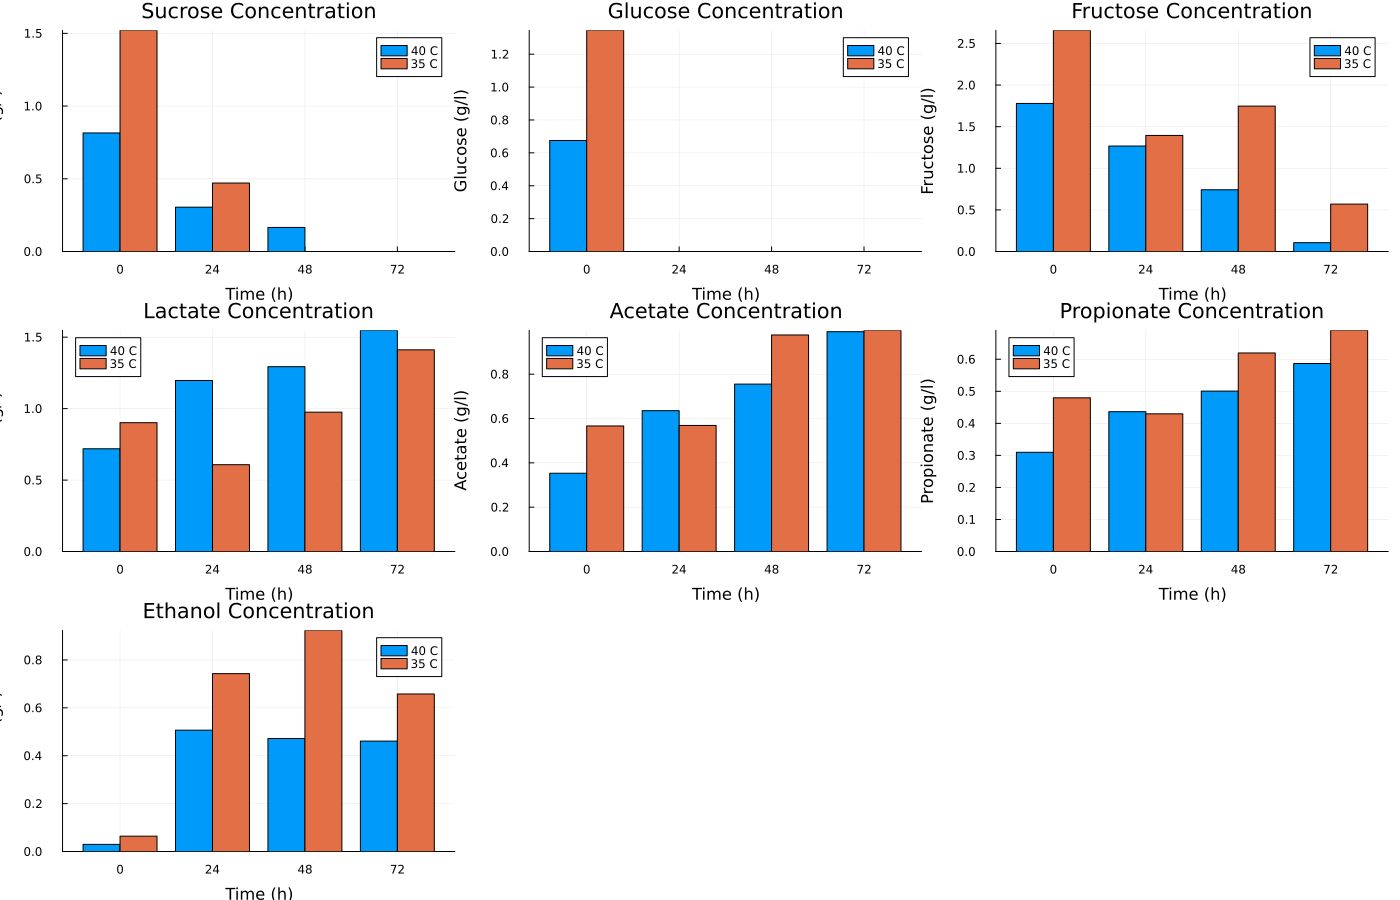
\includegraphics[width=.8\linewidth]{/home/vidianos/Documents/9o_εξάμηνο/Masters_Thesis/plots/35_40_comp/grouped_bar_comp_0.png}
\caption{Συγκριτικά διαγράμματα στα 0 ml mix}
\end{figure}

\begin{figure}[htbp]
\centering
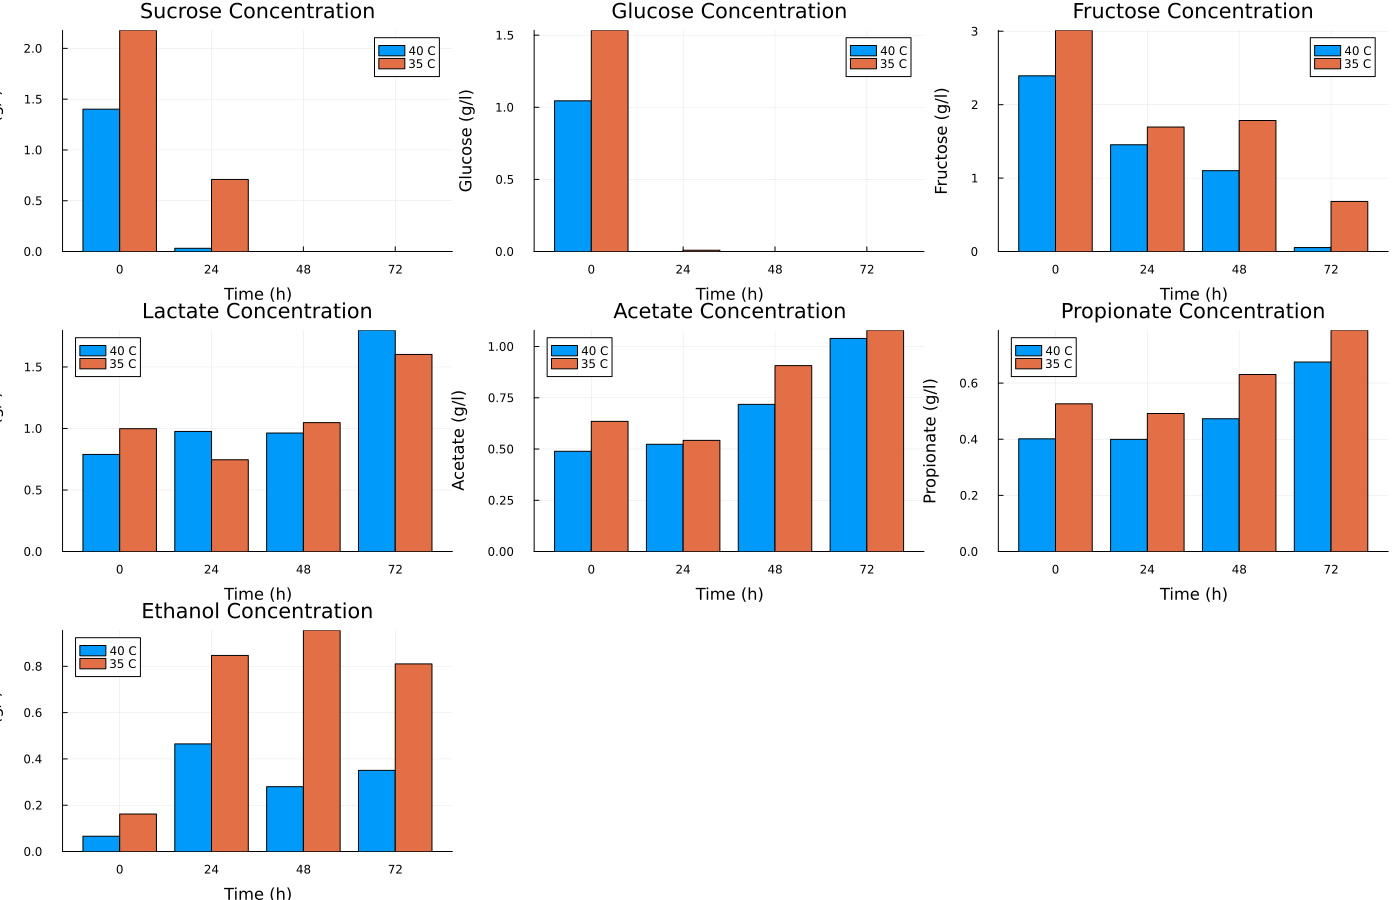
\includegraphics[width=.8\linewidth]{/home/vidianos/Documents/9o_εξάμηνο/Masters_Thesis/plots/35_40_comp/grouped_bar_comp_1.png}
\caption{Συγκριτικά διαγράμματα στα 1 ml mix}
\end{figure}

\begin{figure}[htbp]
\centering
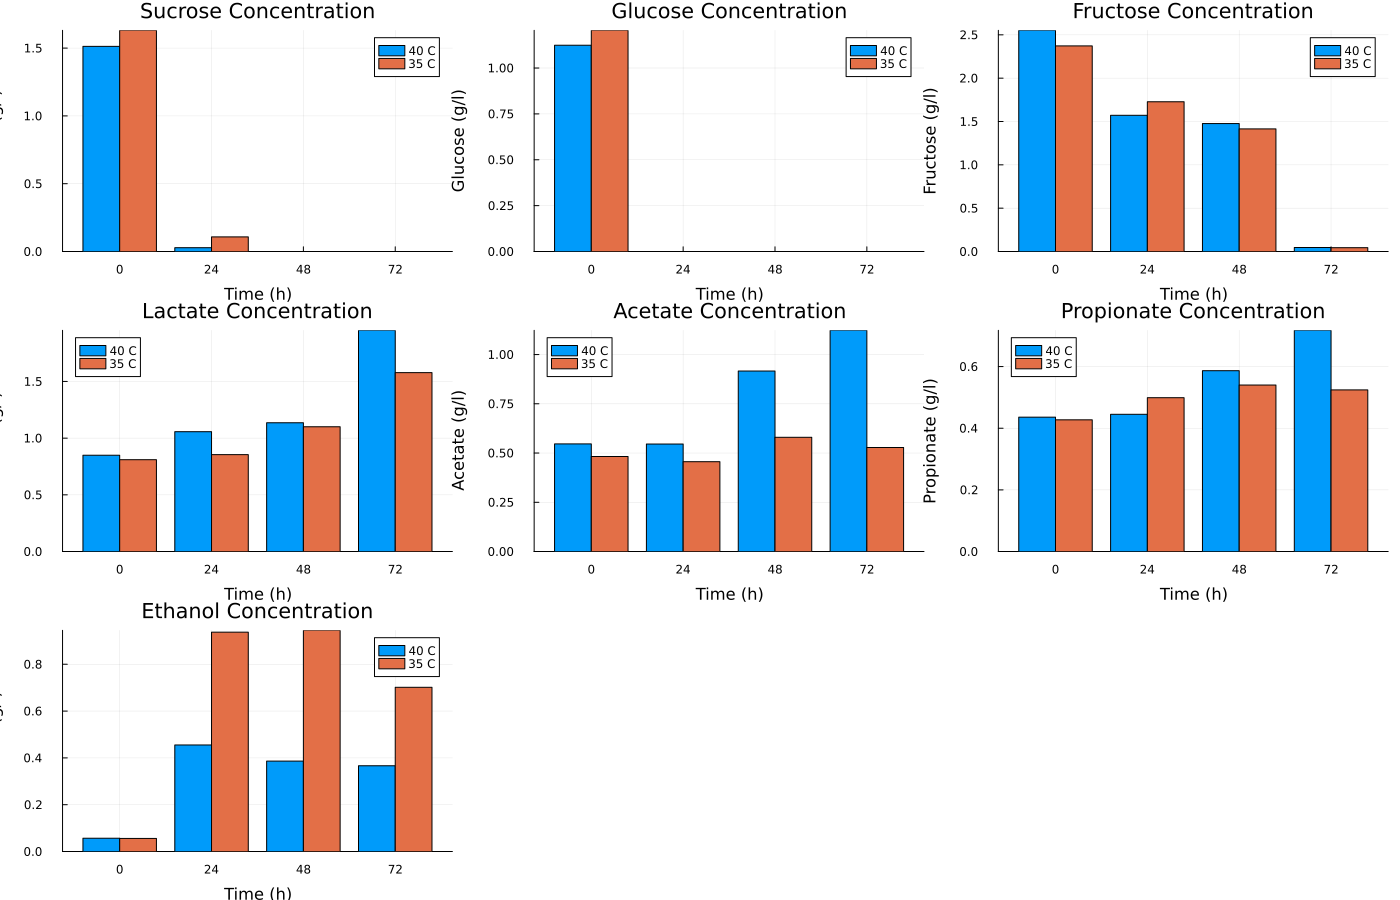
\includegraphics[width=.9\linewidth]{/home/vidianos/Documents/9o_εξάμηνο/Masters_Thesis/plots/35_40_comp/grouped_bar_comp_4.png}
\caption{Συγκριτικά διαγράμματα στα 4 ml mix}
\end{figure}

\begin{figure}[htbp]
\centering
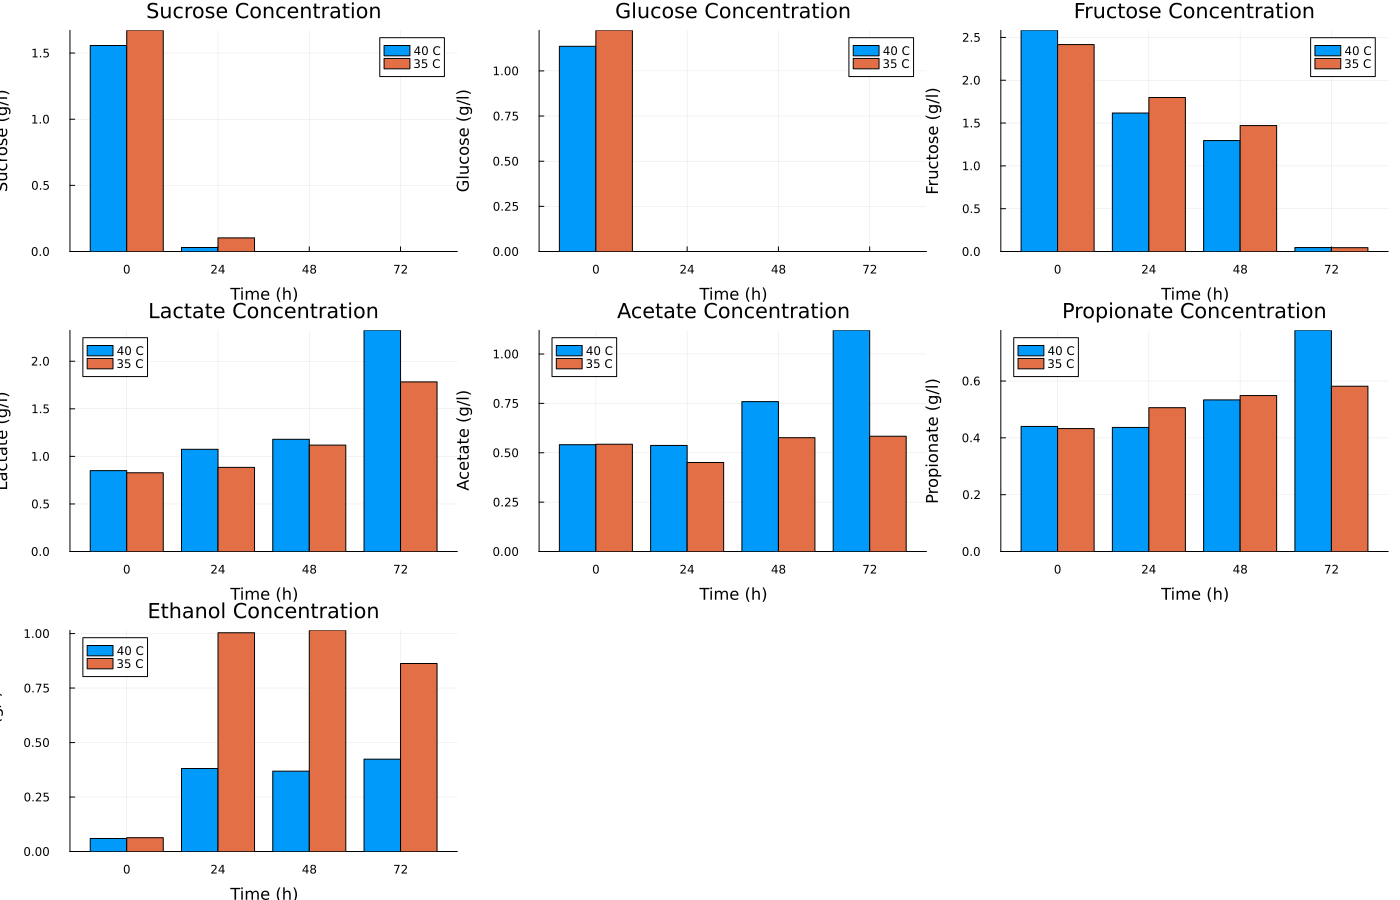
\includegraphics[width=.9\linewidth]{/home/vidianos/Documents/9o_εξάμηνο/Masters_Thesis/plots/35_40_comp/grouped_bar_comp_8.png}
\caption{Συγκριτικά διαγράμματα στα 8 ml mix}
\end{figure}

\pagebreak
\subsection{Τελικό plotting}
\label{sec:org1d42c6b}
Τέλος, ένα code block που τρέχει τα παραπάνω μαζί για να δημιουργήσει τα κατάλληλα διαγράμματα. Αυτό είναι περισσότερο διευκολυντικό για ένα interactive session μέσω του org-mode.

\begin{minted}[breaklines=true,breakanywhere=true]{julia}

<<comp_data_collection>>
<<comp_plots_2_ml>>
<<comp_plots_no_kinetic>>

\end{minted}

\section{Συγκεντρωτικά διαγράμματα σακχάρων και προιόντων}
\label{sec:org0a0daa6}
Τα παραπάνω διαγράμματα είναι χρήσιμα αλλά είναι υπερβολική πληροφορία και πιθανότατα όχι τόσο πρακτική. Για αυτό προτάθηκε να κάνουμε κάποια συγκεντρωτικά διαγράμματα που δείχνουν πως μεταβάλλεται η συγκέντρωση όλων των διαλυτών ενώσεων, των σακχάρων και των προιόντων, συγκεντρωτικά τα οποία μπορεί να μας είναι χρήσιμα. Αρχικά φαίνεται ένα code block το οποίο κάνει την επεξεργασία των data frames για να μαζέψει αυτά τα αθροίσματα.

\textbf{data\textsubscript{analysis}\textsubscript{cumulatives}}
\begin{minted}[breaklines=true,breakanywhere=true]{julia}

df0_total = map(sum, eachrow(df0_conc[:, 2:8]))
df1_total = map(sum, eachrow(df1_conc[:, 2:8]))
df2_total = map(sum, eachrow(df2_conc[:, 2:8]))
df4_total = map(sum, eachrow(df4_conc[:, 2:8]))
df8_total = map(sum, eachrow(df8_conc[:, 2:8]))

df0_sugars = map(sum, eachrow(df0_conc[:, 2:4]))
df1_sugars = map(sum, eachrow(df1_conc[:, 2:4]))
df2_sugars = map(sum, eachrow(df2_conc[:, 2:4]))
df4_sugars = map(sum, eachrow(df4_conc[:, 2:4]))
df8_sugars = map(sum, eachrow(df8_conc[:, 2:4]))

df0_prod = map(sum, eachrow(df0_conc[:, 5:8]))
df1_prod = map(sum, eachrow(df1_conc[:, 5:8]))
df2_prod = map(sum, eachrow(df2_conc[:, 5:8]))
df4_prod = map(sum, eachrow(df4_conc[:, 5:8]))
df8_prod = map(sum, eachrow(df8_conc[:, 5:8]))

\end{minted}

\subsection{Ανάλυση για το πείραμα 23/10}
\label{sec:orgde5ac98}
Λόγω της ιδιαιτερότητας (και μοναδικότητας) του πειράματος αυτού, το dataframe του δεν έχει το generic όνομα αλλά \texttt{df2310} οπότε πρέπει να τρέξουμε το παραπάνω συγκεκριμένα για αυτό το πείραμα.

\textbf{cumulative\textsubscript{analysis}\textsubscript{23}\textsubscript{10}}
\begin{minted}[breaklines=true,breakanywhere=true]{julia}

df2310_1_total = map(sum, eachrow(df2310_1_conc[:, 2:8]))
df2310_2_total = map(sum, eachrow(df2310_2_conc[:, 2:8]))

df2310_1_sugars = map(sum, eachrow(df2310_1_conc[:, 2:4]))
df2310_2_sugars = map(sum, eachrow(df2310_2_conc[:, 2:4]))

df2310_1_prod = map(sum, eachrow(df2310_1_conc[:, 5:8]))
df2310_2_prod = map(sum, eachrow(df2310_2_conc[:, 5:8]))

\end{minted}

\subsection{Δημιουργία διαγραμμάτων}
\label{sec:orgc99b089}
Έπειτα, φαίνεται η δημιουργία των διαγραμμάτων. Προτάθηκε αυτά να γίνουν με scatter plots με γραμμές αντί για bar plots οπότε φαίνεται μόνο αυτό το representation. Για τα file names, όπως και παραπάνω, χρησιμοποιείται το variable \texttt{date} για να ελέγξει για ποιό από τα δύο πειράματα ασχολούμαστε.

\textbf{cumulative\textsubscript{plots}}
\begin{minted}[breaklines=true,breakanywhere=true]{julia}

plot_type = "scatter"
plot_label = ["0 ml" "1 ml" "2 ml" "4 ml" "8 ml"]
colors = ["#009AFA" "#E36F47" "#3EA44E" "#C371D2" "#AC8E18"]

total_conc = plot(t, [df0_total df1_total df2_total df4_total df8_total], title = "Total Concentration",
                  xlabel = "Time (h)", ylabel = "Concentration (g/l)", label = plot_label,
                  linecolor = colors)
scatter!(t, [df0_total df1_total df2_total df4_total df8_total], markersize = 6, label = plot_label,
         markercolor = colors)
savefig(total_conc, get_plot_name("total_conc", date, plot_type))

sugars_conc = plot(t, [df0_sugars df1_sugars df2_sugars df4_sugars df8_sugars], title = "Sugars Concentration",
                  xlabel = "Time (h)", ylabel = "Concentration (g/l)", label = plot_label,
                  linecolor = colors)
scatter!(t, [df0_sugars df1_sugars df2_sugars df4_sugars df8_sugars], markersize = 6, label = plot_label,
         markercolor = colors)
savefig(sugars_conc, get_plot_name("sugars_conc", date, plot_type))

prod_conc = plot(t, [df0_prod df1_prod df2_prod df4_prod df8_prod], title = "Product Concentration",
                  xlabel = "Time (h)", ylabel = "Concentration (g/l)", label = plot_label,
                  linecolor = colors, legend = :topleft)
scatter!(t, [df0_prod df1_prod df2_prod df4_prod df8_prod], markersize = 6, label = plot_label,
         markercolor = colors)
savefig(prod_conc, get_plot_name("product_conc", date, plot_type))

final_plot = plot(sugars_conc, prod_conc, total_conc, size = (1200, 800))
savefig(final_plot, get_plot_name("total_plots", date, plot_type))

\end{minted}

Αντίστοιχα, βάζουμε το code block που φτιάχνει τα plots για το πείραμα στις 23/10. Καθώς μπορεί να μην έχει την σωστή τιμή το date variable, θα γίνει updated για τα plots αυτά (αυτό είναι κυρίως για το interactivity του notebook, στο tangled source σίγουρα θα είναι σωστό το date).

\textbf{cumulative\textsubscript{plots}\textsubscript{23}\textsubscript{10}}
\begin{minted}[breaklines=true,breakanywhere=true]{julia}

date = "23_10"
plot_type = "scatter"

total_conc_2310 = plot(t1, df2310_1_total, title = "Total Concentration",
                       xlabel = "Time (h)", ylabel = "Concentration (g/l)",
                       linecolor = "#009AFA", label = "(1)")
plot!(t2, df2310_2_total, title = "Total Concentration",
      xlabel = "Time (h)", ylabel = "Concentration (g/l)",
      linecolor = "#E36F47", label = "(2)")
scatter!(t1, df2310_1_total, markersize = 6, markercolor = "#009AFA", label = "(1)")
scatter!(t2, df2310_2_total, markersize = 6, markercolor = "#E36F47", label = "(2)")
savefig(total_conc_2310, get_plot_name("total_conc", date, plot_type))

sugars_conc_2310 = plot(t1, df2310_1_sugars, title = "Sugars Concentration",
                          xlabel = "Time (h)", ylabel = "Concentration (g/l)",
                          linecolor = "#009AFA", label = "(1)")
plot!(t2, df2310_2_sugars, title = "Sugars Concentration",
      xlabel = "Time (h)", ylabel = "Concentration (g/l)",
      linecolor = "#E36F47", label = "(2)")
scatter!(t1, df2310_1_sugars, markersize = 6, markercolor = "#009AFA", label = "(1)")
scatter!(t2, df2310_2_sugars, markersize = 6, markercolor = "#E36F47", label = "(2)")
savefig(sugars_conc_2310, get_plot_name("sugars_conc", date, plot_type))

prod_conc_2310 = plot(t1, df2310_1_prod, title = "Product Concentration",
                        xlabel = "Time (h)", ylabel = "Concentration (g/l)",
                        linecolor = "#009AFA", legend = :bottomright,
                        label = "(1)")
plot!(t2, df2310_2_prod, title = "Product Concentration",
      xlabel = "Time (h)", ylabel = "Concentration (g/l)",
      linecolor = "#E36F47", legend = :bottomright,
      label = "(2)")
scatter!(t1, df2310_1_prod, markersize = 6, markercolor = "#009AFA", label = "(1)")
scatter!(t2, df2310_2_prod, markersize = 6, markercolor = "#E36F47", label = "(2)")
savefig(prod_conc_2310, get_plot_name("product_conc", date, plot_type))

final_plot_2310 = plot(sugars_conc_2310, prod_conc_2310, total_conc_2310,
                       size = (1200, 800))
savefig(final_plot_2310, get_plot_name("total_plots", date, plot_type))

\end{minted}

\section{Μετατροπή σακχάρων σε προιόντα}
\label{sec:org3e4e804}
Ακόμη, μία ιδέα που είχαμε είναι η χρήση του λόγου τελικών προιόντων προς αρχικά σάκχαρα ως μία απόκριση του συστήματος για να κρίνουμε ποιό πείραμα ήταν καλύτερο. Επίσης δοκιμάστηκε εκτός από τελικά προιόντα να χρησιμοποιηθεί η μεταβολή προιόντων στον αριθμητή (τελικά - αρχικά προιόντα) για να απεξαρτητοποιηθεί το πείραμα από τις αρχικές ποσότητες. Τα παρακάτω code blocks κάνουν αυτή την ανάλυση. Καθώς εδώ κάθε πείραμα είναι ένα σημείο, είναι πιο εύκολο να μπούν όλα τα πειράματα μαζί, οπότε για να γίνουν θα χρησιμοποιηθούν και κάποια από τα παραπάνω blocks.

Αρχικά, μαζεύουμε τους πίνακες με τα δεδομένα που θέλουμε και κάνουμε την κατάλληλη επεξεργασία

\textbf{sugar\textsubscript{to}\textsubscript{prod}\textsubscript{1}}
\begin{minted}[breaklines=true,breakanywhere=true]{julia}

# 10/11 Experiment
<<area_to_conc_10_11>>
<<data_analysis_cumulatives>>

df0_10_11_conv = df0_prod[4]/df0_sugars[1]
df1_10_11_conv = df1_prod[4]/df1_sugars[1]
df2_10_11_conv = df2_prod[4]/df2_sugars[1]
df4_10_11_conv = df4_prod[4]/df4_sugars[1]
df8_10_11_conv = df8_prod[4]/df8_sugars[1]
conversion_10_11 = [df0_10_11_conv, df1_10_11_conv, df2_10_11_conv, df4_10_11_conv, df8_10_11_conv]

# 28/11 Experiment
<<area_to_conc_28_11>>
<<data_analysis_cumulatives>>

df0_28_11_conv = df0_prod[4]/df0_sugars[1]
df1_28_11_conv = df1_prod[4]/df1_sugars[1]
df2_28_11_conv = df2_prod[4]/df2_sugars[1]
df4_28_11_conv = df4_prod[4]/df4_sugars[1]
df8_28_11_conv = df8_prod[4]/df8_sugars[1]
conversion_28_11 = [df0_28_11_conv, df1_28_11_conv, df2_28_11_conv, df4_28_11_conv, df8_28_11_conv]

# 23/10 Experiment
df2310_1_conv = df2310_1_prod[21]/df2310_1_sugars[1]
df2310_2_conv = df2310_2_prod[17]/df2310_2_sugars[1]
\end{minted}

\subsection{Δημιουργία διαγραμμάτων}
\label{sec:org096a541}
Έπειτα, με τα παραπάνω δεδομένα μπορούμε να φτιάξουμε ξεχωριστά διαγράμματα για το πείραμα 10/11 και 28/11, συγκριτικά τους και ένα συγκριτικό και με τα 3 πειράματα.

Εδώ δεν χρειάζεται χρήση του date καθώς δεν είναι code φτιαγμένο να τρέχει με διαφορετικές ημερομηνίες.

\textbf{sugar\textsubscript{to}\textsubscript{prod}\textsubscript{plots}\textsubscript{1}}
\begin{minted}[breaklines=true,breakanywhere=true]{julia}

sugar_10_11_conv = scatter([0, 1, 2, 3, 4], [conversion_10_11],
                     xticks = (0:4, mix_amount), xlabel = "Amount of mix (ml)",
                     ylabel = "Conversion rate", markersize = 6,
                     title = "Conversion of sugars to products, T = 35 C",
                     legend = false)
savefig(sugar_10_11_conv, plotsdir("10_11/sugar_conv_10_11.png"))

sugar_28_11_conv = scatter([0, 1, 2, 3, 4], [conversion_28_11],
                     xticks = (0:4, mix_amount), xlabel = "Amount of mix (ml)",
                     ylabel = "Conversion rate", markersize = 6,
                     title = "Conversion of sugars to products, T = 40 C",
                     legend = false)
savefig(sugar_28_11_conv, plotsdir("28_11/sugar_conv_28_11.png"))

sugar_conv = scatter([0, 1, 2, 3, 4], [conversion_10_11 conversion_28_11],
                     xticks = (0:4, mix_amount), xlabel = "Amount of mix (ml)",
                     ylabel = "Conversion rate", markersize = 6,
                     title = "Conversion of sugars to products",
                     label = ["35 C" "40 C"])
savefig(sugar_conv, plotsdir("35_40_comp/sugar_conv.png"))

sugar_conv_complete = scatter([0, 1, 2, 3, 4], [conversion_10_11 conversion_28_11],
                              xticks = (0:4, mix_amount), xlabel = "Amount of mix (ml)",
                              ylabel = "Conversion rate", markersize = 6,
                              title = "Conversion of sugars to products",
                              label = ["35 C" "40 C"])
scatter!([2], [df2310_1_conv df2310_2_conv],
         markersize = 6, label = ["45 C (1)" "45 C (2)"])
savefig(sugar_conv_complete, plotsdir("35_40_45_comp/sugar_conv.png"))
\end{minted}

\begin{verbatim}
"/home/vidianos/Documents/9o_εξάμηνο/Masters_Thesis/plots/35_40_45_comp/sugar_conv.png"
\end{verbatim}


\begin{figure}[htbp]
\centering
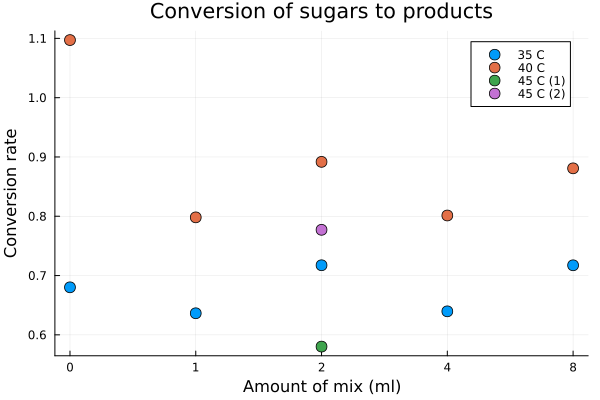
\includegraphics[width=.9\linewidth]{/home/vidianos/Documents/9o_εξάμηνο/Masters_Thesis/plots/35_40_45_comp/sugar_conv.png}
\caption{Λόγος τελικών προιόντων με αρχικά σάκχαρα σε όλα τα πειράματα}
\end{figure}

\subsection{Διαγράμματα με μεταβολή προιόντων}
\label{sec:orgf420f58}
Έπειτα, κάνουμε τα ίδια για μεταβολή προιόντων όπως αναφέρθηκε. Χρειάζεται ένα αντίστοιχο data extraction και ένα plotting με τα παραπάνω.

\textbf{sugar\textsubscript{to}\textsubscript{prod}\textsubscript{2}}
\begin{minted}[breaklines=true,breakanywhere=true]{julia}

# 10/11 Experiment
<<area_to_conc_10_11>>
<<data_analysis_cumulatives>>

sug_to_prod_0 = df0_prod./df0_sugars[1]
Δprod_0 = (last(sug_to_prod_0) - first(sug_to_prod_0))*100

sug_to_prod_1 = df1_prod./df1_sugars[1]
Δprod_1 = (last(sug_to_prod_1) - first(sug_to_prod_1))*100

sug_to_prod_2 = df2_prod./df2_sugars[1]
Δprod_2 = (last(sug_to_prod_2) - first(sug_to_prod_2))*100

sug_to_prod_4 = df4_prod./df4_sugars[1]
Δprod_4 = (last(sug_to_prod_4) - first(sug_to_prod_4))*100

sug_to_prod_8 = df8_prod./df8_sugars[1]
Δprod_8 = (last(sug_to_prod_8) - first(sug_to_prod_8))*100

Δprod_10_11 = [Δprod_0, Δprod_1, Δprod_2, Δprod_4, Δprod_8]

# 28/11 Experiment
<<area_to_conc_28_11>>
<<data_analysis_cumulatives>>

sug_to_prod_0 = df0_prod./df0_sugars[1]
Δprod_0 = (last(sug_to_prod_0) - first(sug_to_prod_0))*100

sug_to_prod_1 = df1_prod./df1_sugars[1]
Δprod_1 = (last(sug_to_prod_1) - first(sug_to_prod_1))*100

sug_to_prod_2 = df2_prod./df2_sugars[1]
Δprod_2 = (last(sug_to_prod_2) - first(sug_to_prod_2))*100

sug_to_prod_4 = df4_prod./df4_sugars[1]
Δprod_4 = (last(sug_to_prod_4) - first(sug_to_prod_4))*100

sug_to_prod_8 = df8_prod./df8_sugars[1]
Δprod_8 = (last(sug_to_prod_8) - first(sug_to_prod_8))*100

Δprod_28_11 = [Δprod_0, Δprod_1, Δprod_2, Δprod_4, Δprod_8]

# 23/10 Experiment
sug_to_prod_2310_1 = df2310_1_prod./df2310_1_sugars[1]
Δprod_2310_1 = (last(sug_to_prod_2310_1) - first(sug_to_prod_2310_1))*100

sug_to_prod_2310_2 = df2310_2_prod./df2310_2_sugars[1]
Δprod_2310_2 = (last(sug_to_prod_2310_2) - first(sug_to_prod_2310_2))*100
\end{minted}

\subsubsection{Plots}
\label{sec:orgeb9d6a4}
\textbf{sugar\textsubscript{to}\textsubscript{prod}\textsubscript{plots}\textsubscript{2}}
\begin{minted}[breaklines=true,breakanywhere=true]{julia}

Δprod_plot_10_11 = scatter([0, 1, 2, 3, 4], [Δprod_10_11],
                     xticks = (0:4, mix_amount), xlabel = "Amount of mix (ml)",
                     ylabel = "Δprod/Sugars (%)", markersize = 6,
                     title = "Change in products divided by sugars T = 35 C",
                     legend = false)
savefig(Δprod_plot_10_11, plotsdir("10_11/Δprod_10_11.png"))

Δprod_plot_28_11 = scatter([0, 1, 2, 3, 4], [Δprod_28_11],
                     xticks = (0:4, mix_amount), xlabel = "Amount of mix (ml)",
                     ylabel = "Δprod/Sugars (%)", markersize = 6,
                     title = "Change in products divided by sugars T = 40 C",
                     legend = false)
savefig(Δprod_plot_28_11, plotsdir("28_11/Δprod_28_11.png"))

Δprod_comp_plot_1 = scatter([0, 1, 2, 3, 4], [Δprod_10_11 Δprod_28_11],
                     xticks = (0:4, mix_amount), xlabel = "Amount of mix (ml)",
                     ylabel = "Δprod/Sugars (%)", markersize = 6,
                     title = "Change in products divided by sugars",
                     label = ["35 C" "40 C"])
savefig(Δprod_comp_plot_1, plotsdir("35_40_comp/Δprod.png"))

Δprod_comp_plot_2 = scatter([0, 1, 2, 3, 4], [Δprod_10_11 Δprod_28_11],
                     xticks = (0:4, mix_amount), xlabel = "Amount of mix (ml)",
                     ylabel = "Δprod/Sugars (%)", markersize = 6,
                     title = "Change in products divided by sugars",
                     label = ["35 C" "40 C"])
scatter!([2], [Δprod_2310_1 Δprod_2310_2], markersize = 6,
         label = ["45 C (1)" "45 C (2)"])
savefig(Δprod_comp_plot_2, plotsdir("35_40_45_comp/Δprod.png"))
\end{minted}

\begin{figure}[htbp]
\centering
\includegraphics[width=.9\linewidth]{/home/vidianos/Documents/9o_εξάμηνο/Masters_Thesis/plots/35_40_45_comp/Δprod.png}
\caption{Λόγος μεταβολής προιόντων προς αρχικά σάκχαρα για όλα τα πειράματα}
\end{figure}

\subsection{Tangling}
\label{sec:org5519665}
Έπειτα, κάνουμε tangle τα code blocks αυτά σε αρχεία sugar\textsubscript{to}\textsubscript{prod} 1 και 2 τα οποία κάνουν τα διαφορετικά approaches, χωρίς φυσικά να παραλείπουμε τα dependencies, ώστε να υπάρχουν και ως source code.

\textbf{sugar\textsubscript{to}\textsubscript{prod}\textsubscript{tangle}\textsubscript{1}}
\begin{minted}[breaklines=true,breakanywhere=true]{julia}

<<dependencies>>
<<sugar_to_prod_1>>
<<sugar_to_prod_plots_1>>

\end{minted}

\textbf{sugar\textsubscript{to}\textsubscript{prod}\textsubscript{tangle}\textsubscript{2}}
\begin{minted}[breaklines=true,breakanywhere=true]{julia}

<<dependencies>>
<<sugar_to_prod_2>>
<<sugar_to_prod_plots_2>>

\end{minted}

\section{Λαμβάνοντας υπόψην την μεταβολή του όγκου}
\label{sec:org0921387}
Κατά την διάρκεια των πειραμάτων γινόντουσαν δειγματοληψίες οι οποίες αφαιρούσαν μία ποσότητα υγρού από το δείγμα, η οποία δεν επιστρεφόταν καθώς το σύστημα είναι batch και όχι συνεχούς λειτουργίας. Επίσης, λόγω των πολυήμερων πειραμάτων, μία ποσότητα νερού εξατμιζόταν και χανόταν όπως ανοίγαμε το καπάκι του μηχανήματος. Έτσι, η αρχική και η τελική κατάσταση δεν είχαν τον ίδιο όγκο το οποίο μπορεί να επηρεάσει τα αποτελέσματα. Κάποιοι πρόχειροι υπολογισμοί δείχνουν πως τα πειράματα που είχαν 4 δειγματοληψίες σύνολο είναι πρακτικά ανεπηρέαστα από αυτό επειδή ο όγκος μειώθηκε το πολύ κατά 50 ml, το οποίο περίπου \(6 \%\) του συνόλου. Στην περίπτωση όμως του αρχικού κινητικού πειράματος όπου ύπηρξαν πολλές δειγματοληψίες, η μεταβολή του όγκου είναι πολύ πιο σημαντική και υπολογίστηκε πως είναι περίπου ένα \(35 \%\) του αρχικού όγκου. Οπότε, εκεί αξίζει να λάβουμε υπόψην την μεταβολή του όγκου και να δούμε τι συμβαίνει σε όρους μάζας και πόσο διαφέρουν από την συγκέντρωση, επειδή εικάζεται πως κάποιες αυξήσεις της συγκέντρωσης οφειλόντουσαν και σε αραίωση του δείγματος.

Αρχικά κάνουμε την προετοιμασία των δεδομένων για αυτό. Για τον υπολογισμό του όγκου κάθε κατάστασης, ξέρουμε περίπου πόσο νερό εξατμίστηκε κατά την διάρκεια του πειράματος από την τελική στάθμη του δοχείου και γνωρίζοντας τον όγκο κάθε δειγματοληψίας (10.5 ml). Υπολογίστηκε πως περίπου 0.675 ml νερό εξατμίζονταν ανά ώρα, το οποίο είναι μία καλή σχετικά προσέγγιση.

\begin{minted}[breaklines=true,breakanywhere=true]{julia}

<<area_to_conc_23_10>>

V1 = [800, 788.83, 777.65, 766.48, 755.3, 744.13, 732.95, 708.95, 697.1, 685.25, 662.6, 650.75, 638.9, 614.9, 603.05, 591.2, 567.2, 555.35, 543.45, 513.45, 500.0]./1000
select!(df2310_1_conc, Not(:Time))
df2310_1_mass = df2310_1_conc.*V1

V2 = [800, 788.83, 775.63, 752.305, 740.46, 728.61, 705.96, 694.11, 682.26, 658.26, 646.41, 634.56, 610.56, 598.71, 586.86, 556.86, 543.56]./1000
select!(df2310_2_conc, Not(:Time))
df2310_2_mass = df2310_2_conc.*V2

df2310_1_total = map(sum, eachrow(df2310_1_mass))
df2310_2_total = map(sum, eachrow(df2310_2_mass))

df2310_1_sugars = map(sum, eachrow(df2310_1_mass[:, 1:3]))
df2310_2_sugars = map(sum, eachrow(df2310_2_mass[:, 1:3]))

df2310_1_prod = map(sum, eachrow(df2310_1_mass[:, 4:7]))
df2310_2_prod = map(sum, eachrow(df2310_2_mass[:, 4:7]))

\end{minted}

\subsection{Δημιουργία των scatter plots}
\label{sec:orgb3fbb4e}
Έπειτα, μπορούμε να κάνουμε τα scatter plots των δύο πειραμάτων χρησιμοποιώντας τα dataframes με τις τιμές μάζας αντί για συγκέντρωσης. Για να διαφοροποιηθούν από τα άλλα στον τίτλο, μπορούμε να βάλουμε στο \texttt{plot\_type} variable την τιμή mass\textsubscript{scatter}.

\begin{minted}[breaklines=true,breakanywhere=true]{julia}

plot_type = "mass_scatter"

suc_scatter = scatter(t1, [df2310_1_conc.Sucrose], label = "1", title = "Sucrose Mass",
                      xlabel = "Time (h)", ylabel = "Sucrose (g)", markersize = 6)
scatter!(t2, df2310_2_conc.Sucrose, label = "2", markersize = 6)
savefig(suc_scatter, get_plot_name("sucrose", date, plot_type))

gluc_scatter = scatter(t1, [df2310_1_conc.Glucose], label = "1", title = "Glucose Mass",
                      xlabel = "Time (h)", ylabel = "Glucose (g)", markersize = 6)
scatter!(t2, df2310_2_conc.Glucose, label = "2", markersize = 6)
savefig(gluc_scatter, get_plot_name("glucose", date, plot_type))

fruc_scatter = scatter(t1, [df2310_1_conc.Fructose], label = "1", title = "Fructose Mass",
                      xlabel = "Time (h)", ylabel = "Fructose (g)", markersize = 6)
scatter!(t2, df2310_2_conc.Fructose, label = "2", markersize = 6)
savefig(fruc_scatter, get_plot_name("fructose", date, plot_type))

lact_scatter = scatter(t1, [df2310_1_conc.Lactate], label = "1", title = "Lactate Mass",
                      xlabel = "Time (h)", ylabel = "Lactate (g)", markersize = 6)
scatter!(t2, df2310_2_conc.Lactate, label = "2", markersize = 6)
savefig(lact_scatter, get_plot_name("lactate", date, plot_type))

ac_scatter = scatter(t1, [df2310_1_conc.Acetate], label = "1", title = "Acetate Mass",
                      xlabel = "Time (h)", ylabel = "Acetate (g)", markersize = 6)
scatter!(t2, df2310_2_conc.Acetate, label = "2", markersize = 6)
savefig(ac_scatter, get_plot_name("acetate", date, plot_type))

prop_scatter = scatter(t1, [df2310_1_conc.Propionate], label = "1", title = "Propionate Mass",
                      xlabel = "Time (h)", ylabel = "Propionate (g)", markersize = 6)
scatter!(t2, df2310_2_conc.Propionate, label = "2", markersize = 6)
savefig(prop_scatter, get_plot_name("propionate", date, plot_type))

eth_scatter = scatter(t1, [df2310_1_conc.Ethanol], label = "1", title = "Ethanol Mass",
                      xlabel = "Time (h)", ylabel = "Ethanol (g)", markersize = 6)
scatter!(t2, df2310_2_conc.Ethanol, label = "2", markersize = 6)
savefig(eth_scatter, get_plot_name("ethanol", date, plot_type))

scatter_final = plot(suc_scatter, gluc_scatter, fruc_scatter,
                         lact_scatter, ac_scatter, prop_scatter,
                         eth_scatter, layout = 9, size = (1350, 900))
savefig(scatter_final, get_plot_name("final", date, plot_type))

\end{minted}

\subsection{Δημιουργία των συγκεντρωτικών plots}
\label{sec:org59843f1}
Έπειτα, μπορούμε να κάνουμε και τα συγκεντρωτικά plots με βάση τα mass data frames ώς εξής.

\begin{minted}[breaklines=true,breakanywhere=true]{julia}

plot_type = "mass"

total_mass_2310 = plot(t1, df2310_1_total, title = "Total Mass",
                       xlabel = "Time (h)", ylabel = "Mass (g)",
                       linecolor = "#009AFA", label = "(1)")
plot!(t2, df2310_2_total, title = "Total Mass",
      xlabel = "Time (h)", ylabel = "Mass (g)",
      linecolor = "#E36F47", label = "(2)")
scatter!(t1, df2310_1_total, markersize = 6, markercolor = "#009AFA", label = "(1)")
scatter!(t2, df2310_2_total, markersize = 6, markercolor = "#E36F47", label = "(2)")
savefig(total_mass_2310, get_plot_name("total", date, plot_type))

sugars_mass_2310 = plot(t1, df2310_1_sugars, title = "Sugars Mass",
                          xlabel = "Time (h)", ylabel = "Mass (g)",
                          linecolor = "#009AFA", label = "(1)")
plot!(t2, df2310_2_sugars, title = "Sugars Mass",
      xlabel = "Time (h)", ylabel = "Mass (g)",
      linecolor = "#E36F47", label = "(2)")
scatter!(t1, df2310_1_sugars, markersize = 6, markercolor = "#009AFA", label = "(1)")
scatter!(t2, df2310_2_sugars, markersize = 6, markercolor = "#E36F47", label = "(2)")
savefig(sugars_mass_2310, get_plot_name("sugars", date, plot_type))

prod_mass_2310 = plot(t1, df2310_1_prod, title = "Product Mass",
                        xlabel = "Time (h)", ylabel = "Mass (g)",
                        linecolor = "#009AFA", legend = :bottomright,
                        label = "(1)")
plot!(t2, df2310_2_prod, title = "Product Mass",
      xlabel = "Time (h)", ylabel = "Mass (g)",
      linecolor = "#E36F47", legend = :bottomright,
      label = "(2)")
scatter!(t1, df2310_1_prod, markersize = 6, markercolor = "#009AFA", label = "(1)")
scatter!(t2, df2310_2_prod, markersize = 6, markercolor = "#E36F47", label = "(2)")
savefig(prod_mass_2310, get_plot_name("product", date, plot_type))

final_plot_2310 = plot(sugars_mass_2310, prod_mass_2310, total_mass_2310,
                       size = (1200, 800))
savefig(final_plot_2310, get_plot_name("total_plots", date, plot_type))

comp_plot_2310 = plot(sugars_conc_2310, prod_conc_2310, total_conc_2310,
                      sugars_mass_2310, prod_mass_2310, total_mass_2310,
                      size = (1200, 800), layout = (2,3))
savefig(comp_plot_2310, get_plot_name("total_comp_conc", date, plot_type))

\end{minted}

\section{Δημιουργία των τελικών διαγραμμάτων}
\label{sec:org1d27d6d}
Τα παραπάνω code blocks όλα υποθέτουν ότι γίνονται executed μετά από το block που διαβάζει τα δεδομένα. Αν θέλουμε, μπορούμε να κάνουμε ένα code block που διαβάζει τα δεδομένα και κάνει sequentially όλα τα plots για κάθε πείραμα, το οποίο μπορεί να είναι και το τελικό μας entry point, είτε για interactive evaluation ή για tangling σε source files.

Ένα μικρό πρόβλημα που υπάρχει είναι πως για κάποιο λόγο το macro \texttt{@quickactivate} δεν λειτουργεί μέσω του org-babel, οπότε αυτά τα code blocks πρέπει να γίνουν tangled ξεχωριστά από τα dependencies για να μην χαθεί το interactivity. Επειδή θέλουμε πάνω πάνω τα dependencies, θα έχουμε πρώτα τα 3 code blocks που κάνουν tangle αυτό και μετά τα executables μου.

\subsection{Dependencies}
\label{sec:org4457c2f}
\begin{minted}[breaklines=true,breakanywhere=true]{julia}
<<dependencies>>
\end{minted}

\begin{minted}[breaklines=true,breakanywhere=true]{julia}
<<dependencies>>
\end{minted}

\begin{minted}[breaklines=true,breakanywhere=true]{julia}
<<dependencies>>
\end{minted}

\subsection{Executables}
\label{sec:org111c85a}
Αυτά τα code blocks τώρα έχουν όλη την πληροφορία και το execution τους παράγει όλα τα plots στο κατάλληλο directory. Για καλύτερο visualization των αποτελεσμάτων, τα τελικά plots που παράγονται παρατίθενται παρακάτω.
\begin{minted}[breaklines=true,breakanywhere=true]{julia}

<<area_to_conc_10_11>>
<<scatter_plots>>
<<conc_scatter_plots>>
<<bar_plots>>
<<conc_bar_plots>>
<<data_analysis_cumulatives>>
<<cumulative_plots>>

\end{minted}

\begin{minted}[breaklines=true,breakanywhere=true]{julia}

<<area_to_conc_28_11>>
<<scatter_plots>>
<<conc_scatter_plots>>
<<bar_plots>>
<<conc_bar_plots>>
<<data_analysis_cumulatives>>
<<cumulative_plots>>

\end{minted}

\begin{minted}[breaklines=true,breakanywhere=true]{julia}

<<scatter_23_10>>
<<cumulative_analysis_23_10>>
<<cumulative_plots_23_10>>

\end{minted}

\begin{minted}[breaklines=true,breakanywhere=true]{julia}

<<23_10_dilution_data_prep>>
<<dilution_scatter_23_10>>
<<dilution_cumulatives_23_10>>

\end{minted}

\subsection{Plots}
\label{sec:org623cae9}
\subsubsection{10/11}
\label{sec:org7018ae2}

\begin{figure}[htbp]
\centering
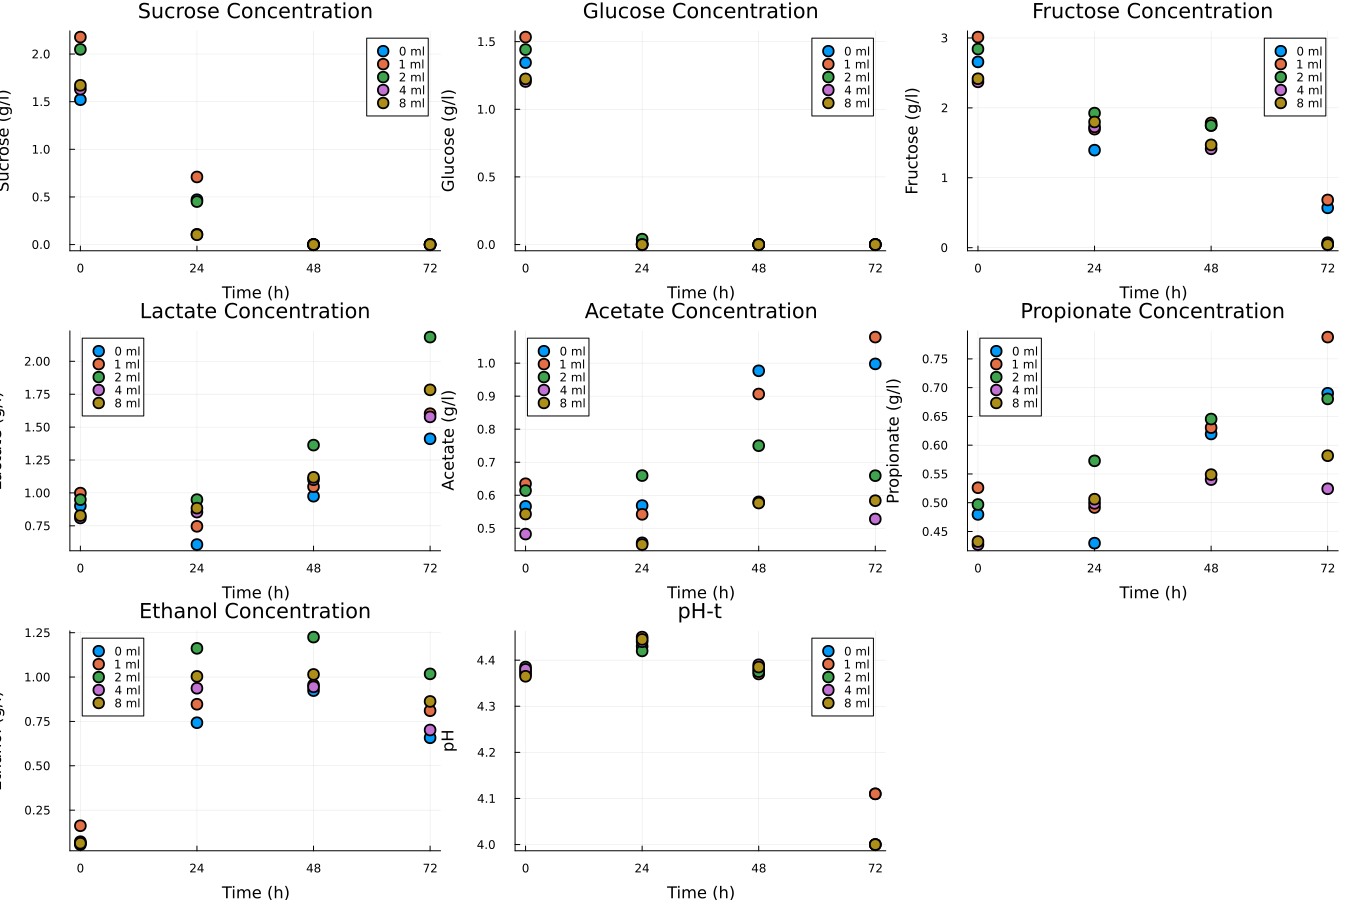
\includegraphics[width=.9\linewidth]{/home/vidianos/Documents/9o_εξάμηνο/Masters_Thesis/plots/10_11/final_scatter_10_11.png}
\caption{Scatter Plots ανά ποσότητα mix}
\end{figure}

\begin{figure}[htbp]
\centering
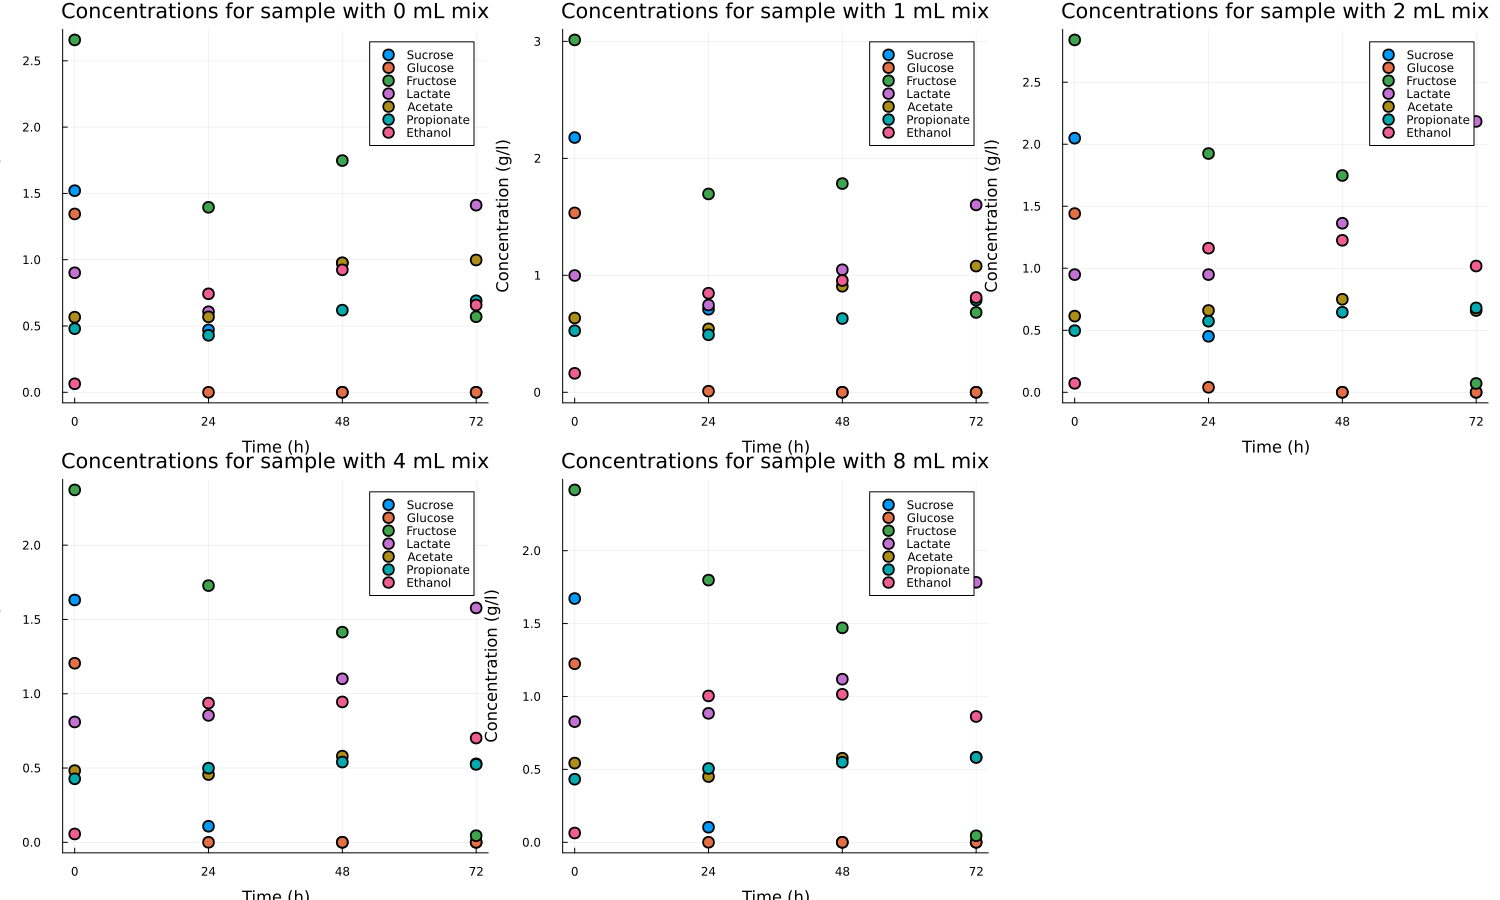
\includegraphics[width=.9\linewidth]{/home/vidianos/Documents/9o_εξάμηνο/Masters_Thesis/plots/10_11/conc_scatter_10_11.png}
\caption{Scatter plots ανά δείγμα}
\end{figure}

\begin{figure}[htbp]
\centering
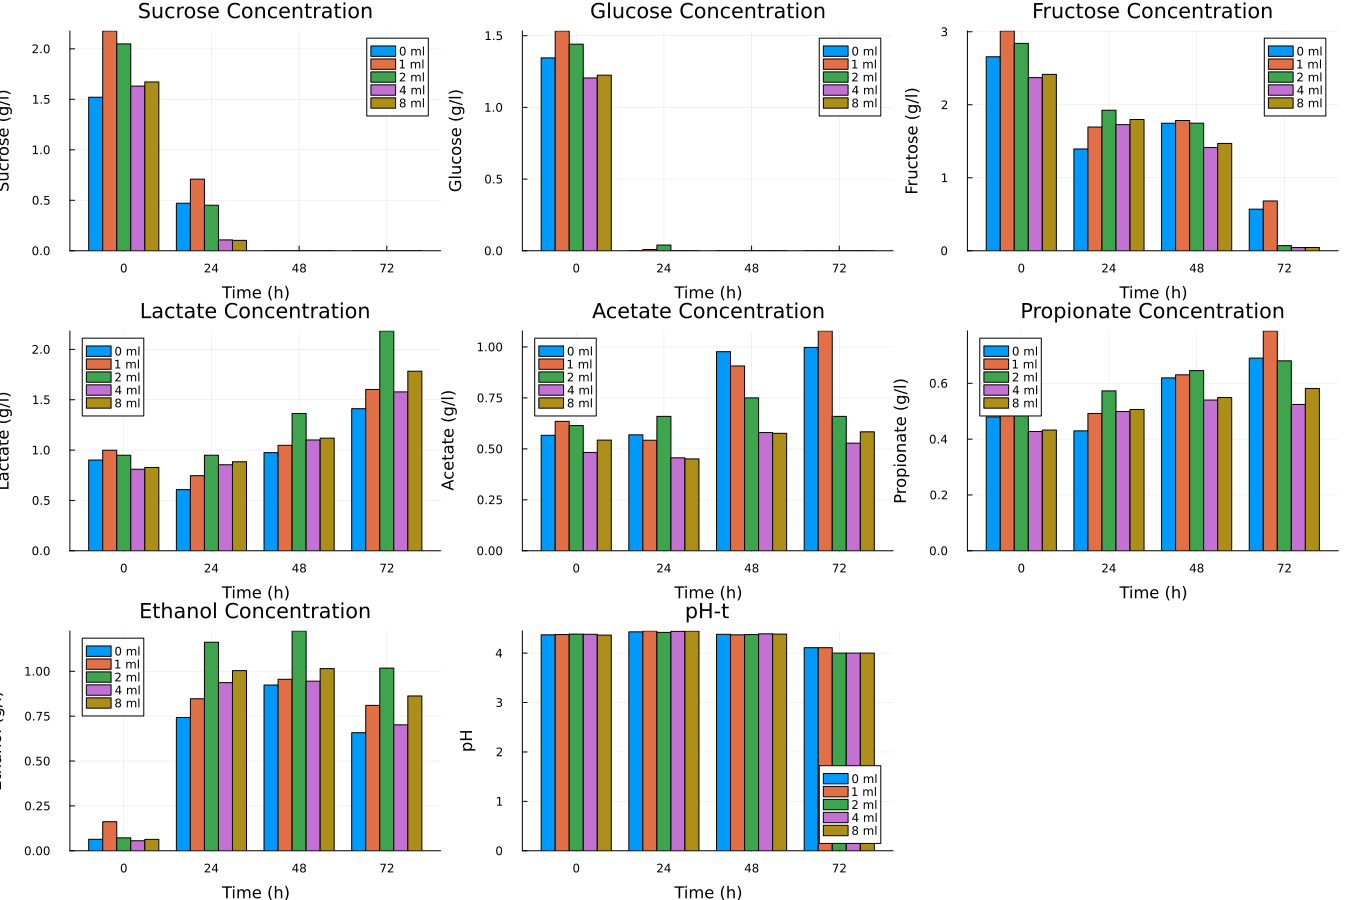
\includegraphics[width=.9\linewidth]{/home/vidianos/Documents/9o_εξάμηνο/Masters_Thesis/plots/10_11/final_bar_10_11.png}
\caption{Bar plots ανά ποσότητα mix}
\end{figure}

\begin{figure}[htbp]
\centering
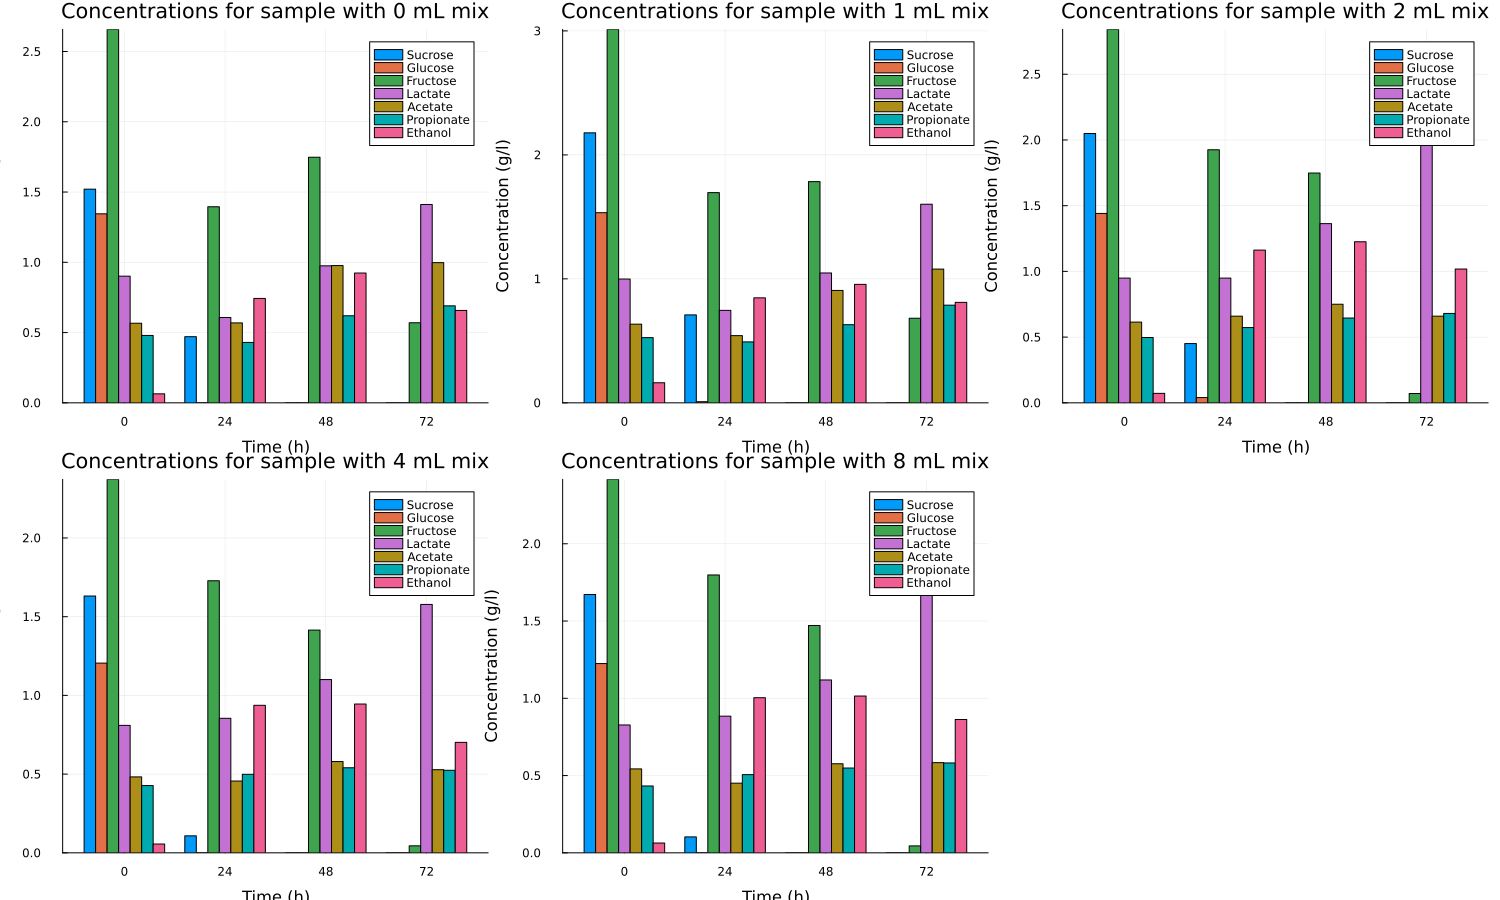
\includegraphics[width=.9\linewidth]{/home/vidianos/Documents/9o_εξάμηνο/Masters_Thesis/plots/10_11/conc_bar_10_11.png}
\caption{Bar plots ανά δείγμα}
\end{figure}

\begin{figure}[htbp]
\centering
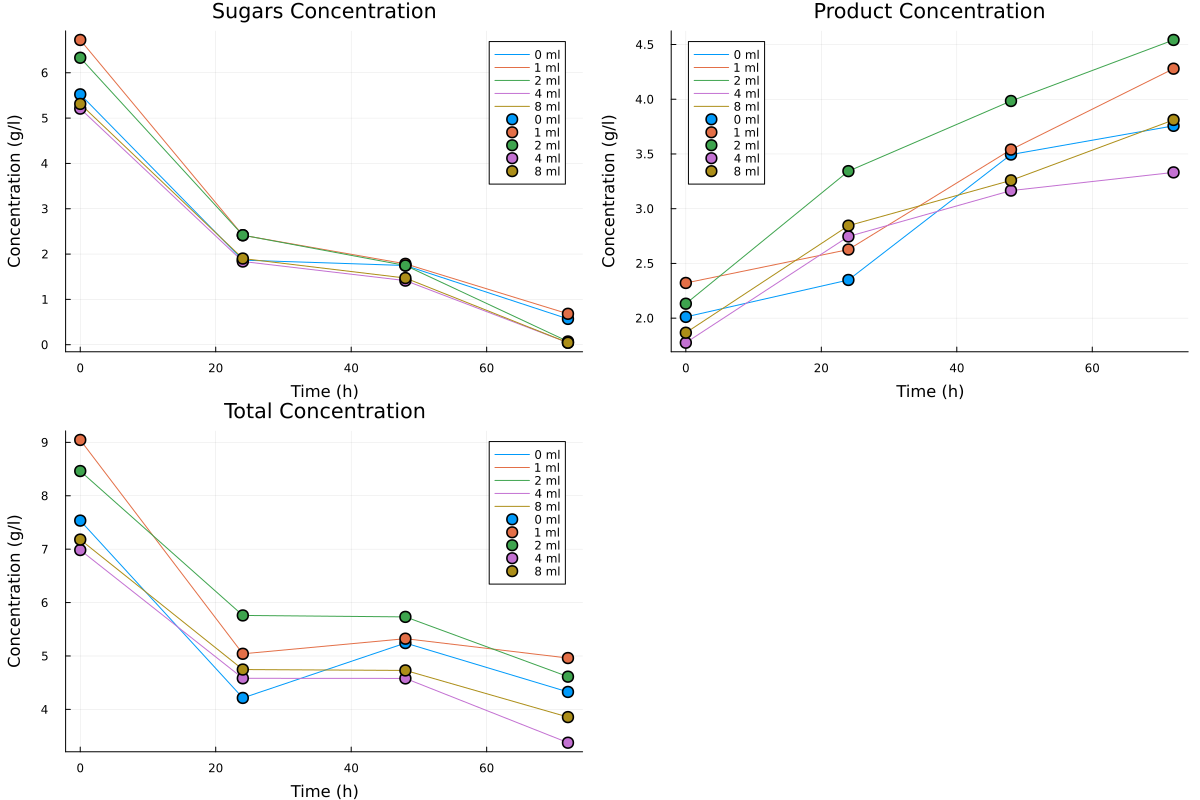
\includegraphics[width=.9\linewidth]{/home/vidianos/Documents/9o_εξάμηνο/Masters_Thesis/plots/10_11/total_plots_scatter_10_11.png}
\caption{Συγκεντρωτικά διαγράμματα}
\end{figure}

\pagebreak

\subsubsection{28/11}
\label{sec:org0ef46ee}

\begin{figure}[htbp]
\centering
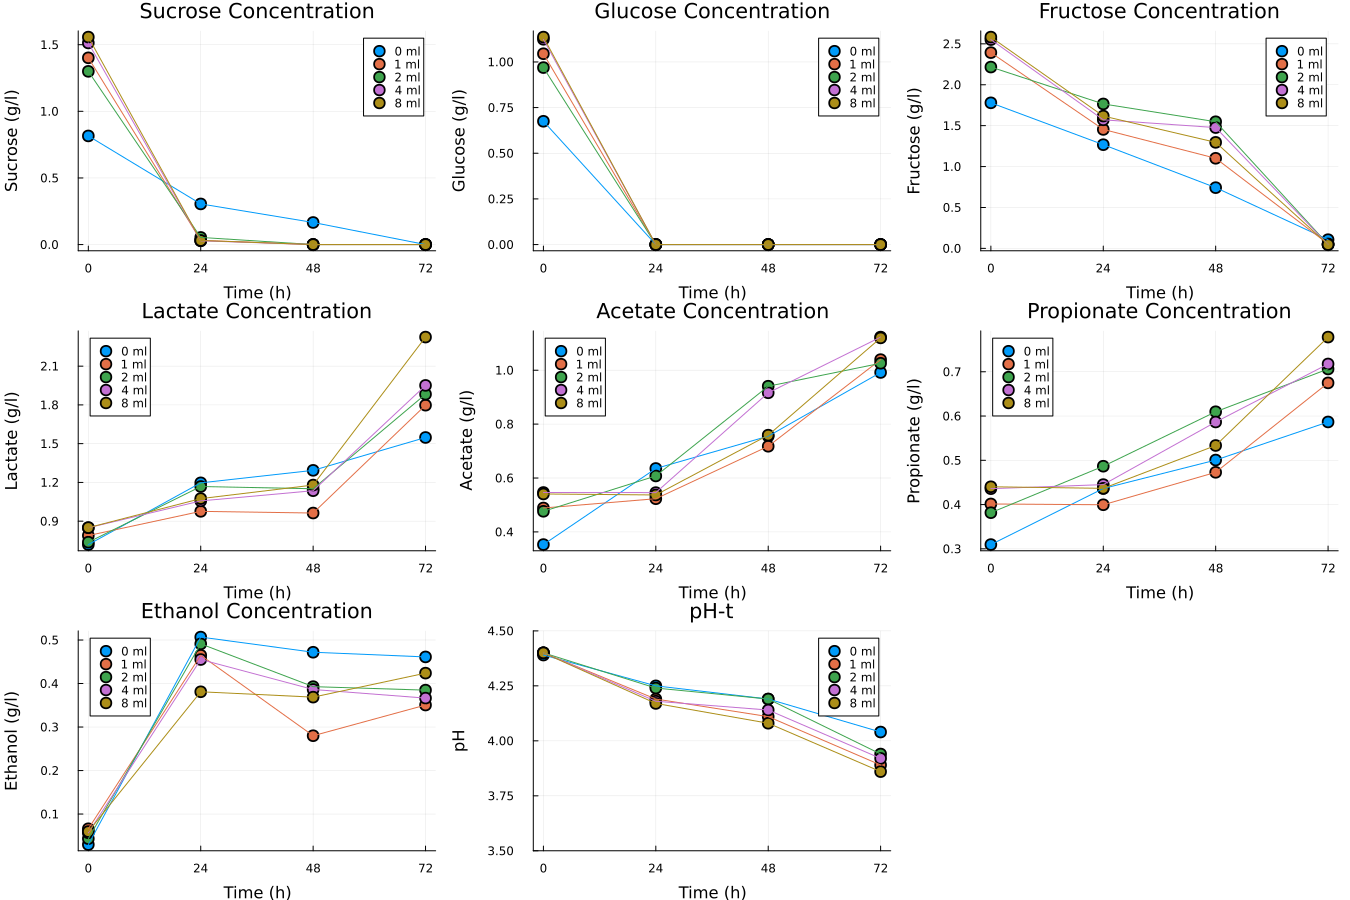
\includegraphics[width=.8\linewidth]{/home/vidianos/Documents/9o_εξάμηνο/Masters_Thesis/plots/28_11/final_scatter_28_11.png}
\caption{Scatter Plots ανά ποσότητα mix}
\end{figure}

\begin{figure}[htbp]
\centering
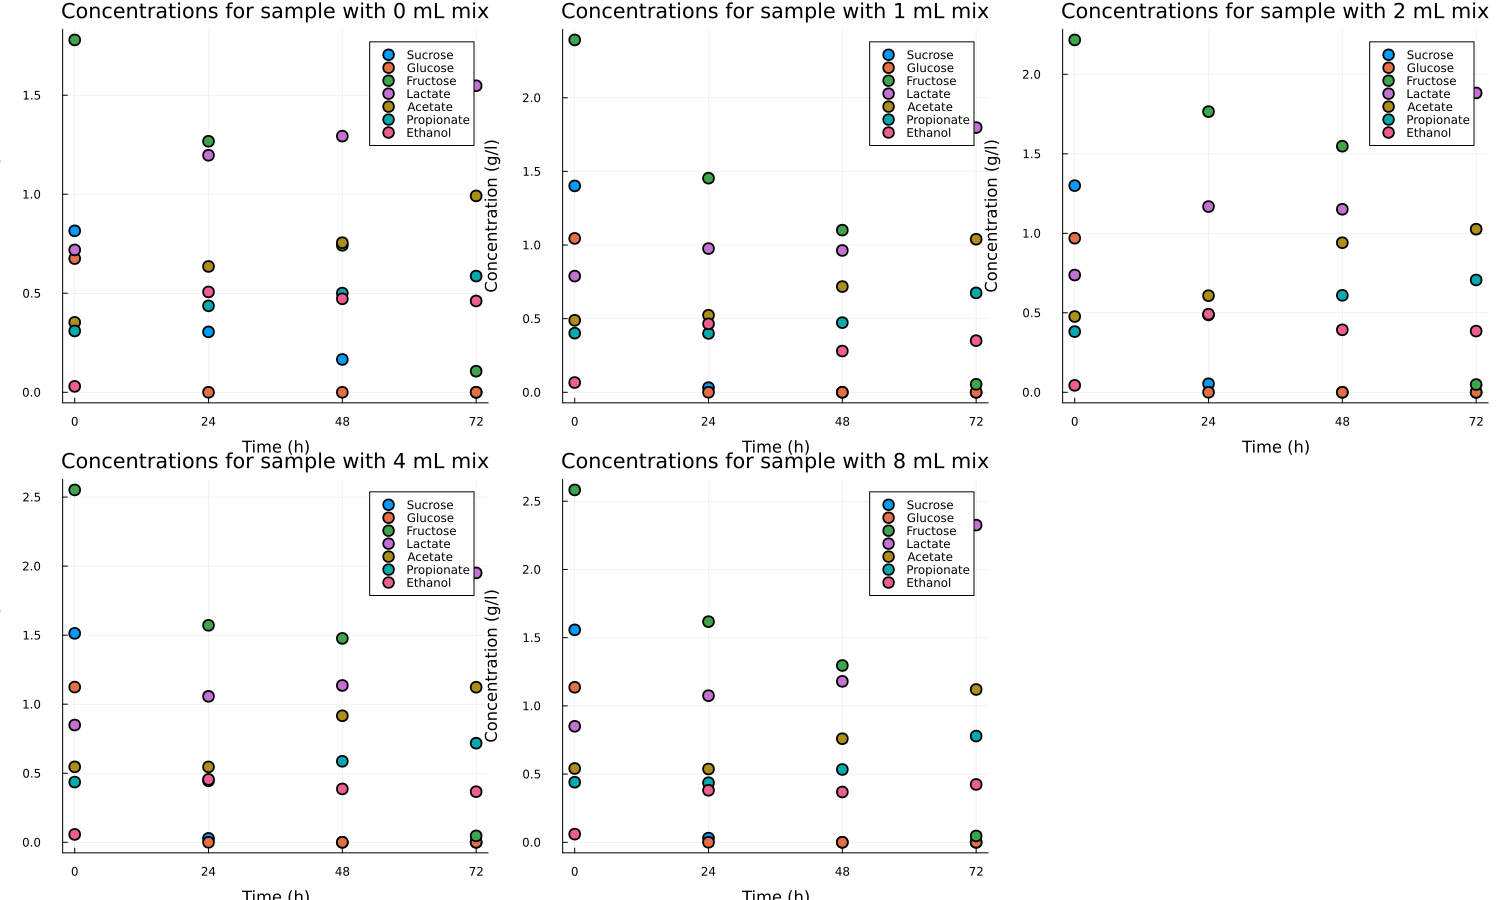
\includegraphics[width=.8\linewidth]{/home/vidianos/Documents/9o_εξάμηνο/Masters_Thesis/plots/28_11/conc_scatter_28_11.png}
\caption{Scatter plots ανά δείγμα}
\end{figure}

\begin{figure}[htbp]
\centering
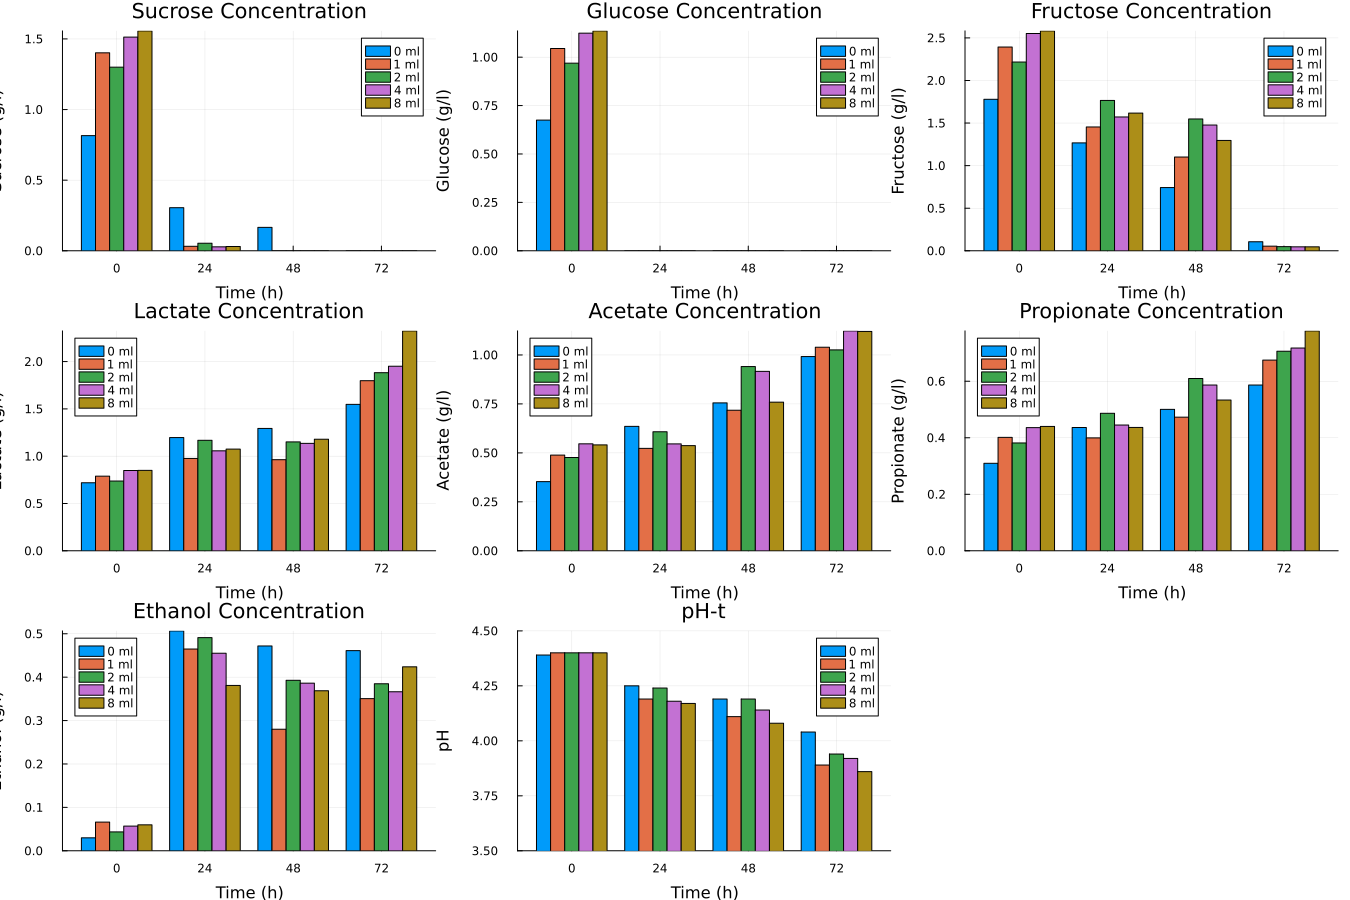
\includegraphics[width=.9\linewidth]{/home/vidianos/Documents/9o_εξάμηνο/Masters_Thesis/plots/28_11/final_bar_28_11.png}
\caption{Bar plots ανά ποσότητα mix}
\end{figure}

\begin{figure}[htbp]
\centering
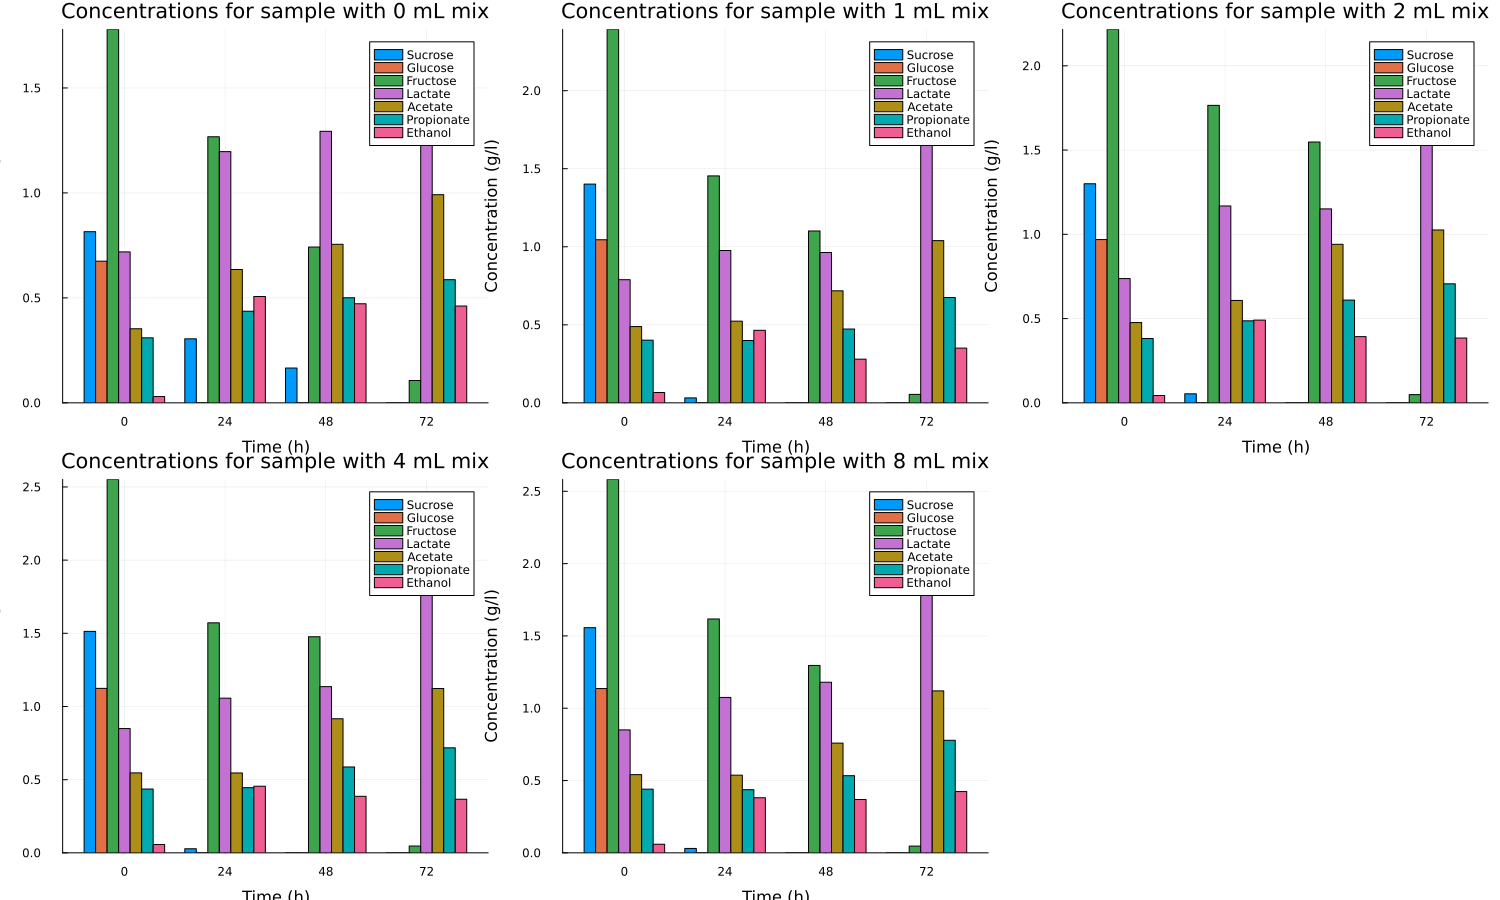
\includegraphics[width=.9\linewidth]{/home/vidianos/Documents/9o_εξάμηνο/Masters_Thesis/plots/28_11/conc_bar_28_11.png}
\caption{Bar plots ανά δείγμα}
\end{figure}

\begin{figure}[htbp]
\centering
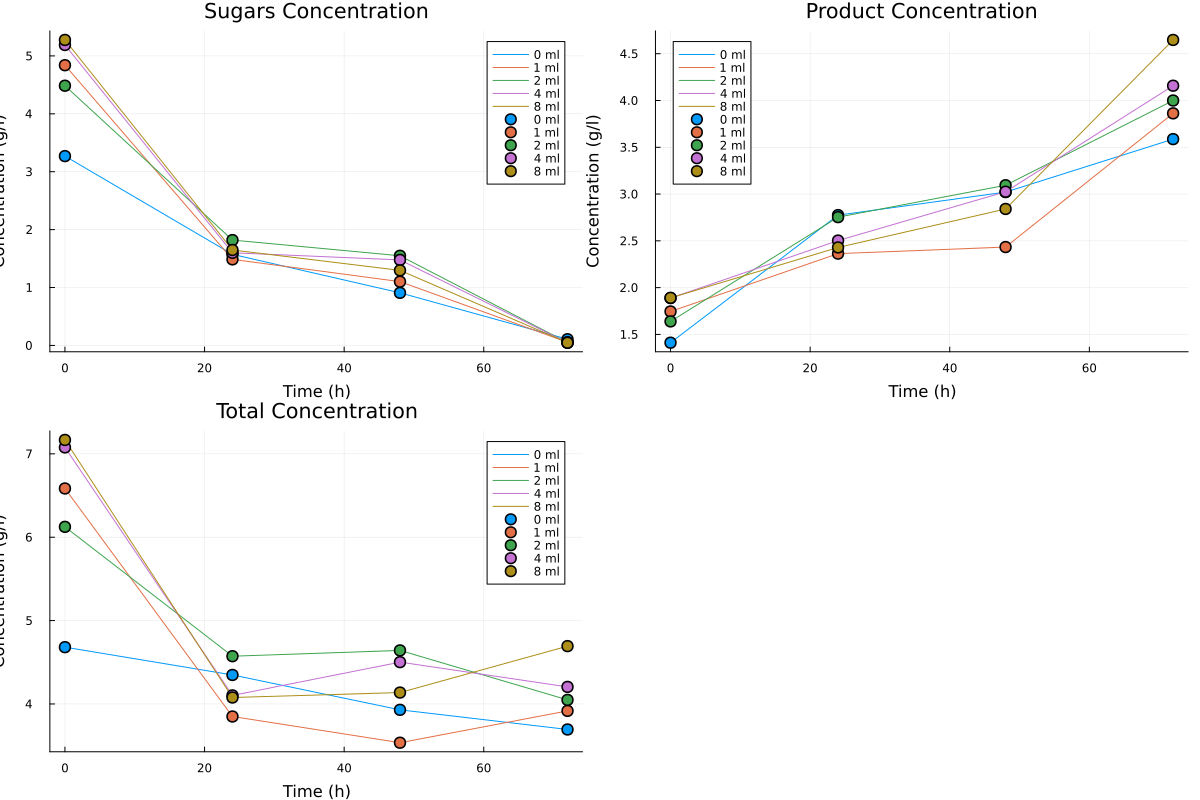
\includegraphics[width=.9\linewidth]{/home/vidianos/Documents/9o_εξάμηνο/Masters_Thesis/plots/28_11/total_plots_scatter_28_11.png}
\caption{Συγκεντρωτικά διαγράμματα}
\end{figure}

\pagebreak
\subsubsection{23/10}
\label{sec:org2b77eae}
\begin{figure}[htbp]
\centering
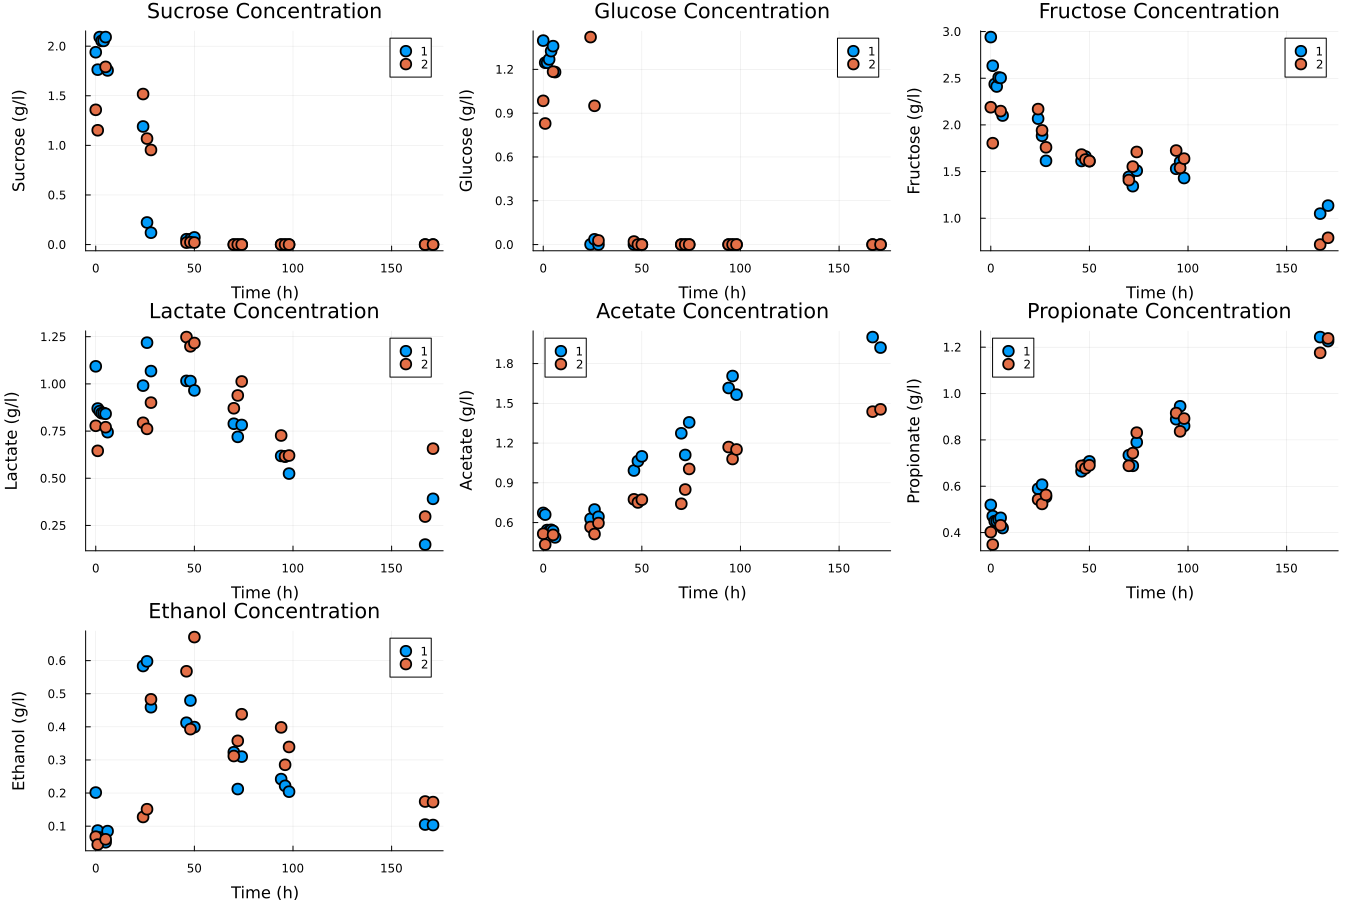
\includegraphics[width=.9\linewidth]{/home/vidianos/Documents/9o_εξάμηνο/Masters_Thesis/plots/23_10/final_scatter_23_10.png}
\caption{Scatter Plots ανά ένωση}
\end{figure}

\begin{figure}[htbp]
\centering
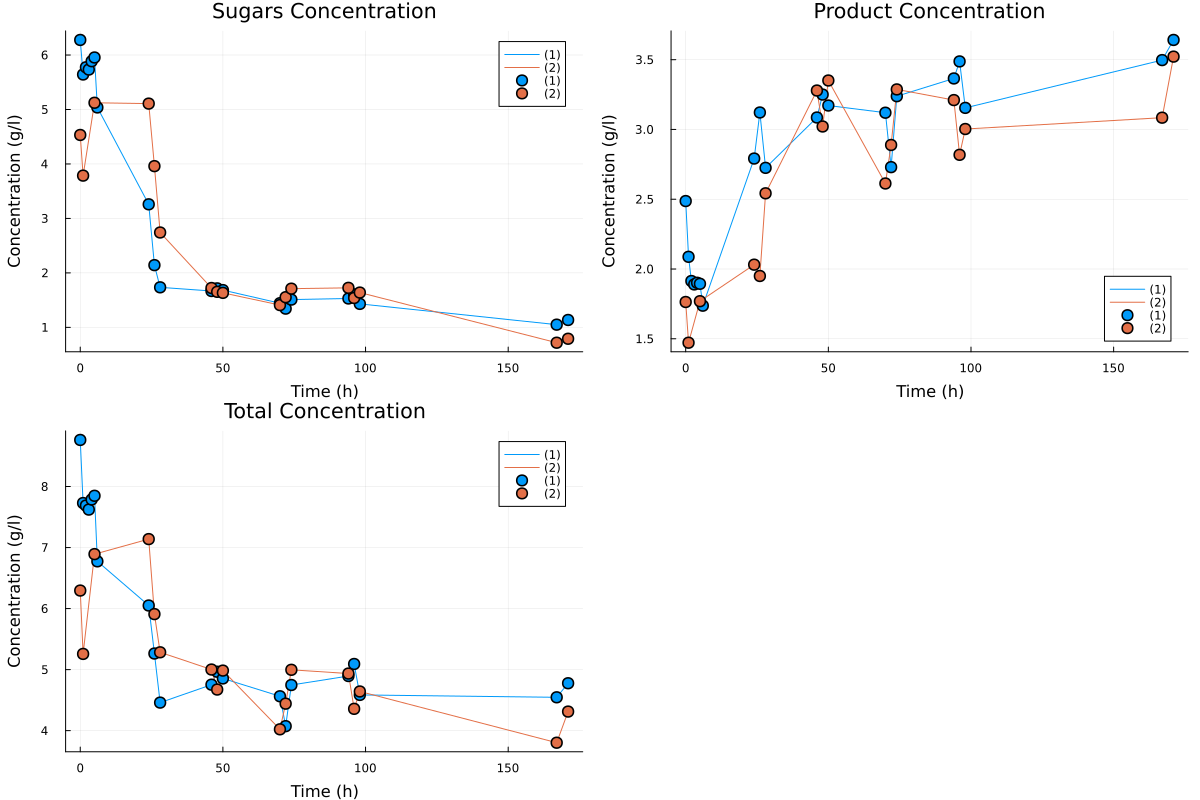
\includegraphics[width=.9\linewidth]{/home/vidianos/Documents/9o_εξάμηνο/Masters_Thesis/plots/23_10/total_plots_scatter_23_10.png}
\caption{Συγκεντρωτικά διαγράμματα}
\end{figure}

\pagebreak
\begin{enumerate}
\item Λαμβάνοντας υπόψην την αραίωση
\label{sec:org89568fe}
\begin{figure}[htbp]
\centering
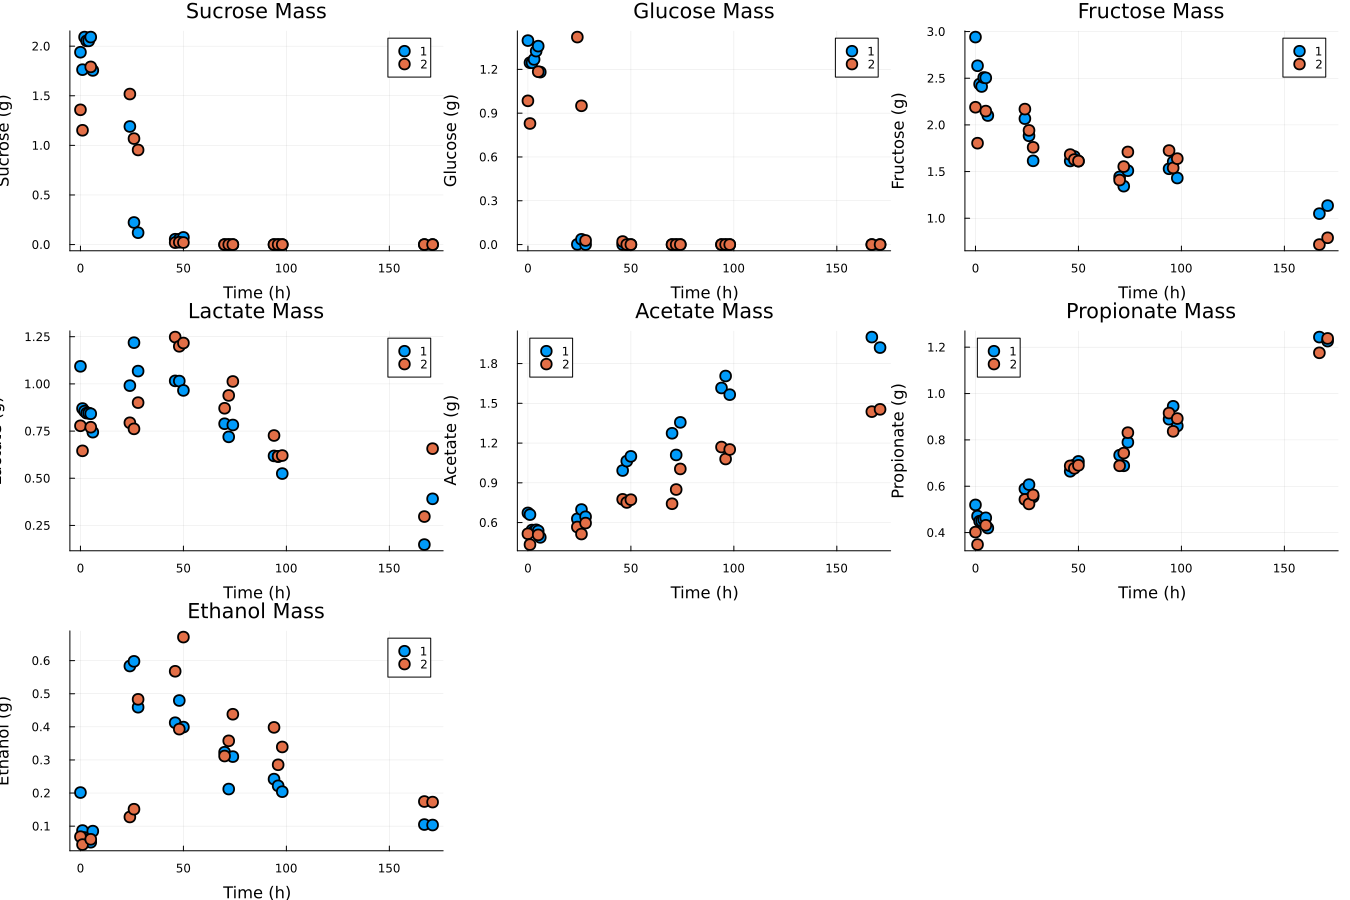
\includegraphics[width=.9\linewidth]{/home/vidianos/Documents/9o_εξάμηνο/Masters_Thesis/plots/23_10/final_mass_scatter_23_10.png}
\caption{Scatter Plots ανά ένωση}
\end{figure}

\begin{figure}[htbp]
\centering
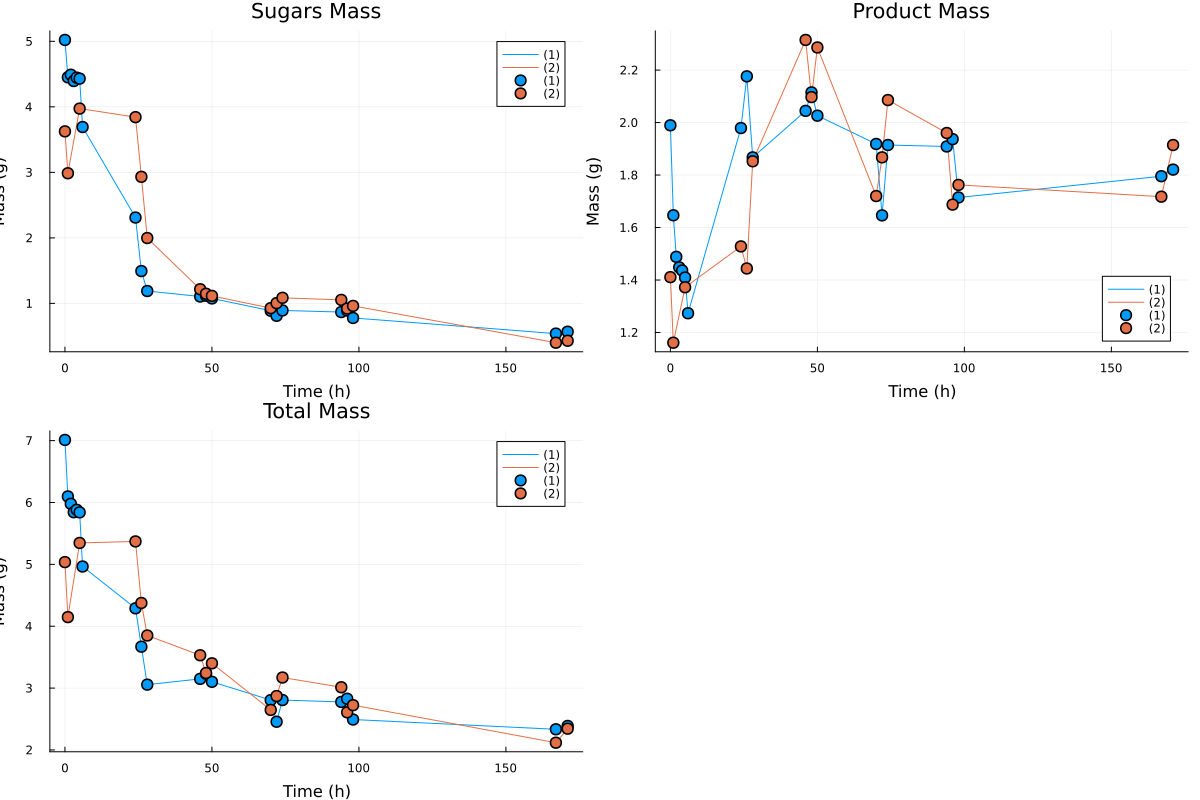
\includegraphics[width=.9\linewidth]{/home/vidianos/Documents/9o_εξάμηνο/Masters_Thesis/plots/23_10/total_plots_mass_23_10.png}
\caption{Συγκεντρωτικά διαγράμματα}
\end{figure}

\begin{figure}[htbp]
\centering
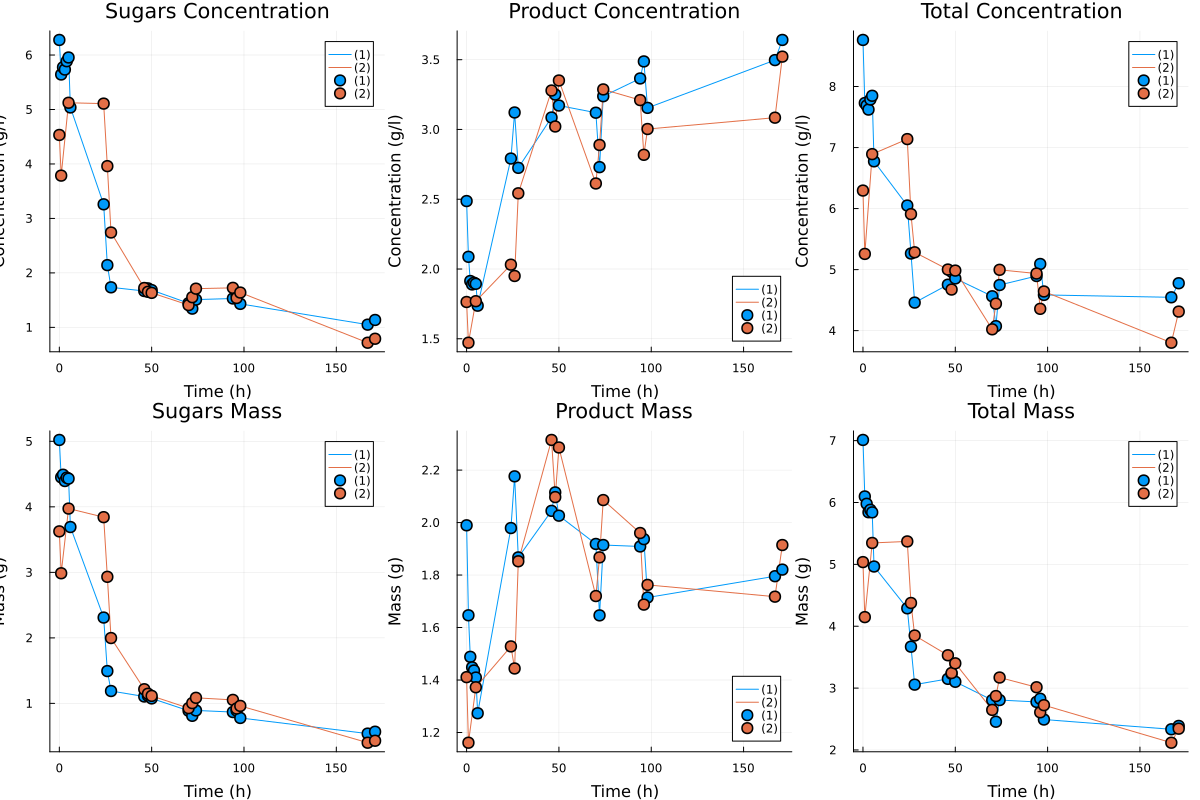
\includegraphics[width=.9\linewidth]{/home/vidianos/Documents/9o_εξάμηνο/Masters_Thesis/plots/23_10/total_comp_conc_mass_23_10.png}
\caption{Σύγκριση συγκεντρωτικών διαγραμμάτων λαμβάνοντας υπόψην την αραίωση ή όχι}
\end{figure}
\end{enumerate}
\end{document}